\ifx\handout\undefined
  \documentclass[compress,t]{beamer}
\else
  \documentclass[compress,handout,t]{beamer}
\fi

\usepackage{amsmath}                  % Nice math stuff
\usepackage{amsfonts}                 % Extra math fonts (i.e., \mathbb{})
\usepackage{amssymb}                  % Extra meth symbols
\usepackage[mathscr]{eucal}           % Scripted math fonts
\usepackage{listings}                 % Formatting code listings
\usepackage{verbatim}
%\usepackage{picins}
\usepackage{colortbl}
\usepackage{fancybox}
\usepackage{textpos}
\usepackage{color}

\mode<presentation>
{
  \usetheme{Warsaw} % or ...
  \setbeamercovered{transparent} % or whatever (possibly just delete it)
  \usefonttheme[onlymath]{serif}
}
\mode<beamer>
{
  \AtBeginSection[]{
    \begin{frame}
      \frametitle{Outline}
      \begin{textblock}{0.9}(0.1,0.0)
        {\small\tableofcontents[currentsection,hideothersubsections]}
      \end{textblock}
    \end{frame}
  }
}
% PKN: the footline isn't very useful -- better to conserve pixels
\setbeamertemplate{footline}{}
\setbeamertemplate{navigation symbols}{}
\setbeamersize{text margin left=0.2cm}
\setbeamersize{text margin right=0.2cm}
\setbeamersize{sidebar width left=0cm}
\setbeamersize{sidebar width right=0cm}
%\setbeamertemplate{footline}
%{% 
%\begin{beamercolorbox}{section in head/foot} 
%\vskip2pt\insertnavigation{\paperwidth}\vskip2pt 
%\vskip2pt
%\hfill Page \insertpagenumber \hspace{1em}
%\end{beamercolorbox}% 
%} 

\usepackage[english]{babel}           % or whatever
\usepackage[latin1]{inputenc}         % or whatever
\usepackage{times}
\usepackage[T1]{fontenc}

\newcommand{\Comment}[1]{{\usebeamercolor[fg]{item}#1}}
\newcommand{\Text}[1]{\texttt{#1}}
\xdefinecolor{TokenColor}{rgb}{0.000, 0.700, 0.000}
\newcommand{\Token}[1]{{\color{TokenColor}#1}}
\xdefinecolor{HiddenColor}{rgb}{0.800, 0.800, 0.800}
\newcommand{\Hidden}[1]{{\color{HiddenColor}#1}}
\xdefinecolor{MyRed}{rgb}{0.800, 0.200, 0.200}
\newcommand{\Red}[1]{{\color{MyRed}#1}}
\xdefinecolor{MyWhite}{rgb}{1.0, 1.0, 1.0}
\xdefinecolor{MyGrey}{rgb}{0.900, 0.900, 0.900}

\setlength{\TPHorizModule}{\textwidth}
\setlength{\TPVertModule}{\textheight}

\lstloadlanguages{C++}
\lstset{%
  basicstyle=\ttfamily\scriptsize\bfseries, %
  commentstyle=\usebeamercolor[fg]{item}, %
  stringstyle=\color{TokenColor}, %
  language=C++}

%% Typeset an example command line input.
%\newcommand{\cmd}[1]{\textbf{\texttt{#1}}}
%\newcommand{\cl}[1]{\$ \textbf{#1}}
%\newcommand{\cls}[1]{\texttt{\scriptsize\$ \textbf{#1}}}
%\newcommand{\clsnp}[1]{\texttt{\scriptsize\textbf{#1}}}
\newcommand{\hilight}{\color{blue}}
\xdefinecolor{MyGreen}{rgb}{0.000, 0.500, 0.000} % green
\newcommand{\nonliteral}[1]{{\color{MyGreen}#1}}
\newcommand{\cmd}[1]{\texttt{\hilight#1}}
\newcommand{\cl}[1]{\$ \cmd{#1}}

%% typset a URL in a uniform way
\newcommand{\Link}[1]{{\usebeamercolor[fg]{item}\underline{\url{#1}}}}

\usepackage{multicol}

\usepackage{tikz}
\usetikzlibrary{arrows,snakes,backgrounds,shapes}
\tikzstyle{commit}=[circle,draw=blue!50,fill=blue!20]
\tikzstyle{redCommit}=[circle,draw=MyRed!50,fill=MyRed!20]
\tikzstyle{orphanCommit}=[black!50,circle,draw=blue!20,fill=blue!10]
\tikzstyle{droppedCommit}=[black!60,circle,draw=MyRed!50,fill=MyRed!20,double]
\tikzstyle{ref}=[rectangle,draw=black!50,fill=black!20]
\tikzstyle{specialRef}=[black!50,rectangle,draw=black!50,fill=black!10]
\tikzstyle{msg}=[tape,tape bend top=none,draw=MyRed!50,fill=MyRed!20]
\tikzstyle{prnt}=[thick,-stealth']
\tikzstyle{oprnt}=[black!50,dotted,-stealth',draw=black!50]
\tikzstyle{bptr}=[thick,-latex']
\tikzstyle{nextmsg}=[thick,-open triangle 45]
\newcommand{\parent}[1]{\char94{#1}}
\newcommand{\ancestor}[1]{\char126{#1}}
\colorlet{myred}{red!90!black} % slightly darker than normal red
\colorlet{myblue}{cyan}        % plain cyan works; might consdier darkening
\colorlet{mygreen}{green!70!black} % slightly darker than normal green

\title{Scaling the Merge Machinery}

\author{Elijah Newren}
\institute{Palantir Technologies}

%\date{January 8, 2014}
%\date{Palantir Technologies}
\date{}

%\includeonlyframes{wip}

\begin{document}

%%%%%%%%%%%%%%%%%%%%%%%%%%%%%%%%%%%%%%%%%%%%%%%%%%%%%%%%%%%%%%%%%%%%%%%%%%

\begin{frame}
  \titlepage
  %\mode<handout>{
  %\vfill
  %\begin{center}\scriptsize
  %  \Link{http://wiki.yojoe.local/ITOOLS/git-tutorial}
  %  \vfill
  %  \cmd{git clone gerrit:itools/public/git-tutorial}
  %\end{center}
  %{\tiny\Hidden{\input{VERSION-FILE}}}
  %}
\end{frame}

\title{Git Merge}
\begin{frame}
  \titlepage
\end{frame}

\title{(Git Merge)$^2$}
\begin{frame}
  \titlepage
\end{frame}

%%%%%%%%%%%%%%%%%%%%%%%%%%%%%%%%%%%%%%%%%%%%%%%%%%%%%%%%%%%%%%%%%%%%%%%%%%
\section[Scope]{``Merge machinery'' scope and plans}
%%%%%%%%%%%%%%%%%%%%%%%%%%%%%%%%%%%%%%%%%%%%%%%%%%%%%%%%%%%%%%%%%%%%%%%%%%

\begin{comment}
\subsection{Division}
\begin{frame}
  \frametitle{Division}

  \begin{itemize}[<+->]

    \item xdiff/xmerge.c: 3-way content merging of a single file
    \item ll-merge.c: thin xdl\_merge wrapper; heeds path-specific
          .gitattributes such as special drivers or normalization

    \item merge-recursive.c (default strategy and main engine): finds
          and pre-merges merge-bases, handles path based-conflicts,
          mode-based conflicts (e.g. symlink vs. submodule),
          renames, and wires everything together.
      % merge-recursive is about 2x the size of the other three pieces combined

    \item builtin/merge.c: which strategy (octopus, fast-forward,
          default), diffstat, etc.
  \end{itemize}

\end{frame}
\end{comment}

%%%%%%%%%%%%%%%%%%%%%%%%%%%%%%%%%%%%%%%%%%%%%%%%%%%%%%%%%%%%%%%%%%%%%%%%%%

\subsection{Affected Commands}
\begin{frame}
  \frametitle{Affected Commands}

  The merge machinery (merge-recursive) powers several aspects of git:

  \begin{itemize}[<+->]
    \item merge
    \item cherry-pick
    \item revert
    \item rebase
    \item am -3
    \item stash
    \item checkout -m
  \end{itemize}

\end{frame}

%%%%%%%%%%%%%%%%%%%%%%%%%%%%%%%%%%%%%%%%%%%%%%%%%%%%%%%%%%%%%%%%%%%%%%%%%%

\subsection{Redesign/Rewrite}
\begin{frame}
  \frametitle{Quotes}

  The two most prolific authors of git opining on merge-recursive:

  \only<2->{
  \begin{itemize}

    \item ``[It is] some pretty hairy code.  Every time I
            start to look at it I get confused and can't remember what
            breakthrough I thought I was close to making before.''
            %
            \href{https://public-inbox.org/git/20110616210551.GA15505@sigill.intra.peff.net/}{(Jeff King)}

    \only<3>{
    \item ``I've written off that code as mostly unsalvageable long
            time ago.''
          \href{https://public-inbox.org/git/xmqqk1ydkbx0.fsf@gitster.mtv.corp.google.com/}{(Junio Hamano)}
    }

  \end{itemize}
  }

\end{frame}

%%%%%%%%%%%%%%%%%%%%%%%%%%%%%%%%%%%%%%%%%%%%%%%%%%%%%%%%%%%%%%%%%%%%%%%%%%

\begin{frame}
  \frametitle{Goals}

  Goals for my rewrite of the machinery:
  \begin{itemize}
    \item Maintainability \& understandability
    \item Improved API, enable new features
    \item Correctness
    \item Performance
  \end{itemize}

\end{frame}

%%%%%%%%%%%%%%%%%%%%%%%%%%%%%%%%%%%%%%%%%%%%%%%%%%%%%%%%%%%%%%%%%%%%%%%%%%

\subsection[Perf Strategies]{Performance Strategies}
\begin{frame}
  \frametitle{Performance Strategies}

  \only<1-6>{
  I have always enjoyed performance talks; they make me feel smarter:
  \only<2->{
  \begin{itemize}
    \item Squeezing performance out of the hardware
    \only<3->{
    \item Applying ideas from other problem domains to new areas
    \only<4->{
    \item Using clever approximation algorithms to get near solutions
    \only<5->{
    \item Inventing new algorithms
    }}}
  \end{itemize}
  \only<6>{
    \begin{minipage}{\textwidth}
      \vspace*{-7.5em}
      
\begin{tikzpicture}
        \draw[red,line width=3pt] ( 0,0) -- (11,2.2);
        \draw[red,line width=3pt] (11,0) -- ( 0,2.2);
      \end{tikzpicture}
    \end{minipage}
  }
  }}

  \only<7->{
  Actual performance strategies used:
  \only<8->{
  \begin{itemize}
    \item Avoid well-known slow constructs
    \only<9->{
    \item Don't do unnecessary work
    \only<10->{
    \item Don't redo work
    \only<11->{
    \item Don't redo unnecessary work
    \only<12->{
    \item Fudge "unnecessary"
    }}}}
  \end{itemize}
  }}

\end{frame}

%%%%%%%%%%%%%%%%%%%%%%%%%%%%%%%%%%%%%%%%%%%%%%%%%%%%%%%%%%%%%%%%%%%%%%%%%%

\subsection{Warning}
\begin{frame}
  \frametitle{Warning}

  \vfill
  \begin{center}
    \begin{minipage}{0.55\textwidth}
    \begin{itemize}
      \item Glossing over lots of details
      \item Simplifications not fully accurate
    \end{itemize}
    \end{minipage}
  \end{center}
\end{frame}

%%%%%%%%%%%%%%%%%%%%%%%%%%%%%%%%%%%%%%%%%%%%%%%%%%%%%%%%%%%%%%%%%%%%%%%%%%
\section[Simple Wins]{Simple Performance Wins}
%%%%%%%%%%%%%%%%%%%%%%%%%%%%%%%%%%%%%%%%%%%%%%%%%%%%%%%%%%%%%%%%%%%%%%%%%%

\begin{frame}[fragile]
  \frametitle{Avoiding well-known slow constructs}

  From string-list.h:
  {\scriptsize
  \vspace*{-0.5\baselineskip}
  \begin{verbatim}
 * NOTE: It is more efficient to build an unsorted list and sort it
 * afterwards, instead of building a sorted list (`O(n log n)` instead of
 * `O(n^2)`).
  \end{verbatim}
  \vspace*{-\baselineskip}
  }

  \only<2>{
  Oops.
  }
\end{frame}

%%%%%%%%%%%%%%%%%%%%%%%%%%%%%%%%%%%%%%%%%%%%%%%%%%%%%%%%%%%%%%%%%%%%%%%%%%

\begin{frame}[fragile]
  \frametitle{Avoiding well-known slow constructs}

  Comment above \texttt{remove\_marked\_cache\_entries()}:
  {\scriptsize
  \vspace*{-0.5\baselineskip}
  \begin{verbatim}
/*
 * Remove all cache entries marked for removal...this is much more
 * effective than calling remove_index_entry_at() for each entry to be
 * removed.
 */
  \end{verbatim}
  }

  \only<2->{
  \vspace*{-1.25\baselineskip}
  \begin{itemize}
    \item merge-recursive's design incompatible with this, instead:
    \item O($tracked\_files$) work required for each deletion/insertion
    \item O($2*files\_changed$) deletions/insertions
  \end{itemize}
  }

  \only<3->{
    Needed a significant restructure to avoid this quasi-quadratic
    behavior.
  }

\end{frame}

%%%%%%%%%%%%%%%%%%%%%%%%%%%%%%%%%%%%%%%%%%%%%%%%%%%%%%%%%%%%%%%%%%%%%%%%%%

\begin{frame}[fragile]
  \frametitle{Avoiding unnecessary work}

  \begin{block}{How merge-recursive got its name}
    {\scriptsize
    \begin{semiverbatim}
      static struct commit* merge_recursive_internal(...)
      \{
          ...
          \uncover<2>{
          /* If we have multiple merge bases, merge them together first. */
          \only<1-2>{combined_mb = bases[0];}
          \only<3->{\color{red}combined_mb = bases[0];}
          for (base in bases[1:]) \{
              call_depth++;
              discard_index(repo->index);
              combined_mb = merge_recursive_internal(combined_mb, base);
              call_depth--;
          \}
          \only<1-2>{
          discard_index(repo->index);
          if (!call_depth)
              repo_read_index(opt->repo);
          }
          \only<3->{\color{red}
          discard_index(repo->index);
          if (!call_depth)
              repo_read_index(opt->repo);
          }
          }
          result = merge_trees_internal(combined_mb, side1, side2);
          ...
      \}
    \end{semiverbatim}
    }
  \end{block}

  \only<3>{What if there is only one merge base to start? }\only<4>{Oops.}

\end{frame}

%%%%%%%%%%%%%%%%%%%%%%%%%%%%%%%%%%%%%%%%%%%%%%%%%%%%%%%%%%%%%%%%%%%%%%%%%%

\begin{frame}
  \frametitle{Avoiding redoing work}

  Tree walking from merge-recursive.c:
  \begin{itemize}
    \only<2->{
    \item unpack\_trees()
    \only<3->{
    \item diff to find renames from base->side1
    \only<4->{
    \item diff to find renames from base->side2
    \only<5->{
    \item get all file and directory names on side1
    \only<6->{
    \item get all file and directory names on side2
    \only<7->{
    \item 6x get stage data \only<8->{for EACH rename\only<9->{on EACH side}}
    }}}}}}
  \end{itemize}
  \only<10->{Total: $5+6*#renames$}

  \only<11->{
  Tree traversals from rewritten :
  \begin{itemize}
    \only<12->{
    \item collect\_merge\_info()
    \only<13->{
    \item unpack\_trees()
    }}
  \end{itemize}
  \only<14->{Total: $2$}

\end{frame}

%%%%%%%%%%%%%%%%%%%%%%%%%%%%%%%%%%%%%%%%%%%%%%%%%%%%%%%%%%%%%%%%%%%%%%%%%%

\begin{frame}
  \frametitle{The big kicker...}

  \begin{center}
  \begin{minipage}{0.5\textwidth}
    All of these optimizations combined are often a drop in a bucket
    compared to the cost of rename detection.
  \end{minipage}
  \end{center}

\end{frame}

%%%%%%%%%%%%%%%%%%%%%%%%%%%%%%%%%%%%%%%%%%%%%%%%%%%%%%%%%%%%%%%%%%%%%%%%%%
\section[Background]{Background}
%%%%%%%%%%%%%%%%%%%%%%%%%%%%%%%%%%%%%%%%%%%%%%%%%%%%%%%%%%%%%%%%%%%%%%%%%%

%%%%%%%%%%%%%%%%%%%%%%%%%%%%%%%%%%%%%%%%%%%%%%%%%%%%%%%%%%%%%%%%%%%%%%%%%%
\subsection{Content merge}
%%%%%%%%%%%%%%%%%%%%%%%%%%%%%%%%%%%%%%%%%%%%%%%%%%%%%%%%%%%%%%%%%%%%%%%%%%

\begin{frame}
  \frametitle{Three-way content merge}

  \vspace*{-\baselineskip}
  \begin{multicols}{2}
    File from branch Side1:\\
    {\footnotesize\texttt{%
    %\vspace*{-0.125\baselineskip}%
    \quad{}...                             \\
    \quad{}speak\_like\_a\_pirate(arrrgs); \\
    \quad{}\only<3->{\color{myred}}explore\_sea(aye, matey);\only<3->{\color{black}}\\
    \quad{}shiver(me.timbers);             \\
    %\vspace*{-0.25\baselineskip}%
    \quad{}...                             \\
    }}
    \columnbreak
    \pause
    Same file from branch Side2:\\
    {\footnotesize\texttt{%
    %\vspace*{-0.125\baselineskip}%
    \quad{}...                             \\
    \quad{}speak\_like\_a\_pirate(arrrgs); \\
    \quad{}\only<3->{\color{myred}}explore\_sea(me.love[0]);\only<3->{\color{black}}\\
    \quad{}shiver(me.timbers);             \\
    %\vspace*{-0.5\baselineskip}%
    \quad{}...
    }}
  \end{multicols}%

  \only<4->{
    \vspace{-0.5\baselineskip}
    Correct merge depends on the version in the merge base:\\
    {\footnotesize\texttt{%
      \quad{}speak\_like\_a\_pirate(arrrgs);\\
      \quad{}%
      \only<4>{{\color{myblue}?????}}%
      \only<5-6>{{\color{myblue}explore\_sea(aye, matey);}}%
      \only<7-8>{{\color{myblue}explore\_sea(me.love[0]);}}%
      \only<9->{{\color{myblue}explore\_sea(plus, plus);}}%
      \\
      \quad{}shiver(me.timbers);\\
    }}
  }

  \only<6-10>{
  \vspace*{0.5\baselineskip}
  Which results in the following merge:\\
  {\footnotesize\texttt{%
    \quad{}speak\_like\_a\_pirate(arrrgs);\\
    \quad{}%
    \only<7,9>{\qquad}%
    \only<6>{{\color{mygreen}explore\_sea(me.love[0]);}}%
    \only<8>{{\color{mygreen}explore\_sea(aye, matey);}}%
    \only<10>{{\color{mygreen}
    <{}<{}<{}<{}<{}<{}< HEAD  \\
    \quad{}explore\_sea(aye, matey); \\
    \quad{}=======\\
    \quad{}explore\_sea(me.love[0]); \\
    \quad{}>{}>{}>{}>{}>{}>{}> branchB
    }}
    \\
    \quad{}shiver(me.timbers);\\
  }}
  }

  \only<11->{
    \vspace*{-0.5\baselineskip}
    \begin{multicols}{2}
      Shorthand:\\
      {\footnotesize\texttt{%
      \quad{}\phantom{Base1: }path\\
      \quad{}Base\phantom{1}: hash\_orig\\
      \quad{}Side1: hash\_A\\
      \quad{}Side2: hash\_B\\
      }}
    \columnbreak
    \uncover<12->{
      Example:\\
      {\footnotesize\texttt{%
      \quad{}\phantom{Base1: }buccaneer.c\\
      \quad{}Base\phantom{1}: ba771ed\\
      \quad{}Side1: 57abbed\\
      \quad{}Side2: b1a57ed
      }}
    }
    \end{multicols}%
  }

  \only<13>{
    \vspace*{-0.5\baselineskip}
    {\footnotesize%
    
      Note: If any two of the hashes match, we can resolve without
      looking at the contents of the file.
      
    }
  }

\end{frame}

%%%%%%%%%%%%%%%%%%%%%%%%%%%%%%%%%%%%%%%%%%%%%%%%%%%%%%%%%%%%%%%%%%%%%%%%%%
\subsection{Basic Merging}
%%%%%%%%%%%%%%%%%%%%%%%%%%%%%%%%%%%%%%%%%%%%%%%%%%%%%%%%%%%%%%%%%%%%%%%%%%

%%%%%%%%%%%%%%%%%%%%%%%%%%%%%%%%%%%%%%%%%%%%%%%%%%%%%%%%%%%%%%%%%%%%%%%%%%

\begin{frame}
  \frametitle{Three-way Merging}

  \cl{git checkout master}\\
  \cl{git merge feature}\\[0.5em]

  \uncover<3->{
  Get three relevant trees}\uncover<4->{, then for each path:
  \begin{itemize}
    \item Get version of path in each tree
    \item Do three-way content merge
  \end{itemize}
  }

  %\only<1| handout:1>{Initial state:}
  %\only<2| handout:2>{\cl{git fetch}}
  %\only<3-4| handout:3>{\cl{git merge origin/master}}
  %\only<5| handout:4>{\cl{git push}}
  \vspace*{-1.5em}

  \pause
  \begin{center}
    \begin{minipage}{0.5\textwidth}
    \begin{block}{Merge}
      \begin{tikzpicture}[node distance=10mm]
        \only<2->{
          \node[commit] (Z) {Z};
        }
        \only<2,6>{
          \node[commit] (Y)  [right of=Z] {Y};
          \node[commit] (W)  [right of=Y] {W};
          \node[commit] (X)  [below right of=Z,yshift=-1em] {X};
        }
        \only<3-5>{
          \node[orphanCommit] (Y)  [right of=Z] {Y};
          \node[orphanCommit] (W)  [right of=Y] {W};
          \node[orphanCommit] (X)  [below right of=Z,yshift=-1em] {X};
        }
        \only<2->{
          \node[commit] (V)  [right of=W] {V};
          \path[prnt] (V) edge (W);
          \path[prnt] (W) edge (Y);
          \path[prnt] (Y) edge (Z);

          \node[commit] (U)  [right of=X] {U};
          \path[prnt] (U) edge (X);
          \path[prnt] (X) edge (Z);

          \node[ref]    (f) [below of=U] {feature};
          \path[bptr] (f) edge (U);
          \node[ref]    (m)  [above of=V] {master};
        }

        \only<2-5| handout:1>{
          \path[bptr] (m) edge (V);
        }
        \only<5>{
          \node[redCommit] (T)  [right of=V] {T};
        }
        \only<6>{
          \node[commit] (T)  [right of=V] {T};
        }
        \only<5-| handout:2-3>{
          \path[prnt] (T) edge (V);
          \path[prnt] (T) edge[bend left] (U);
        }
        \only<6>{
          \path[bptr] (m) edge (T);
        }
      \end{tikzpicture}
    \end{block}
    \end{minipage}
  \end{center}

\end{frame}

%%%%%%%%%%%%%%%%%%%%%%%%%%%%%%%%%%%%%%%%%%%%%%%%%%%%%%%%%%%%%%%%%%%%%%%%%%

\begin{frame}[fragile]
  \frametitle{Three-way Merging}

  \cl{git checkout master}\\
  \cl{git cherry-pick X..feature}\\[0.5em]

  \vspace*{-1.5em}
  \begin{center}
    \begin{minipage}{0.5\textwidth}
    \begin{block}{
        \only<1>{Starting state}
        \only<2-4>{Picking U}
        \only<5>{Picked U}
        \only<6-8>{Picking T}
        \only<9>{Picked T}
        \only<10->{Cherry picking complete}
        \phantom{Cg}% To make sure all titles have the same height
        }
      \begin{tikzpicture}[node distance=10mm]
        \only<1->{
          \node[commit] (Z) {Z};
          \node[commit] (Y)  [right of=Z] {Y};
          \node[commit] (W)  [right of=Y] {W};
          \node[commit] (V)  [right of=W] {V};
          \node[commit] (X)  [below right of=Z,yshift=-1em] {X};
          \node[commit] (U)  [right of=X] {U};
          \node[commit] (T)  [right of=U] {T};
        }
        \only<3-7>{
          \node[orphanCommit] (Z)  {Z};
          \node[orphanCommit] (Y)  [right of=Z] {Y};
          \node[orphanCommit] (W)  [right of=Y] {W};
          \node[orphanCommit] (T)  [right of=U] {T};
        }
        \only<1->{
          \path[prnt] (V) edge (W);
          \path[prnt] (W) edge (Y);
          \path[prnt] (Y) edge (Z);

          \path[prnt] (T) edge (U);
          \path[prnt] (U) edge (X);
          \path[prnt] (X) edge (Z);

          \node[ref]  (f) [below of=T] {feature};
          \path[bptr] (f) edge (T);
          \node[ref]  (m) [above of=V] {master};
        }

        \only<1-9| handout:1>{
          \path[bptr] (m) edge (V);
          %\node[ref]    (h)  [left of=m,xshift=-1.8em] {HEAD};
          %\path[bptr] (h) edge (m);
        }
        \only<4>{
          \node[redCommit] (US) [right of=V, xshift=0.1em] {U$^*$};
          \path[oprnt] (US) edge[bend left] (U);
        }
        \only<4-| handout:2-3>{
          \path[prnt] (US) edge (V);
        }
        \only<5->{
          \node[commit] (Z) {Z};
          \node[commit] (Y)  [right of=Z] {Y};
          \node[commit] (W)  [right of=Y] {W};
          \node[commit] (US) [right of=V, xshift=0.1em] {U$^*$};
          \node[commit] (U)  [right of=X] {U};
          \node[commit] (T)  [right of=U] {T};
        }
        \only<7-8>{
          \node[orphanCommit] (Z) {Z};
          \node[orphanCommit] (Y)  [right of=Z] {Y};
          \node[orphanCommit] (W)  [right of=Y] {W};
          \node[orphanCommit] (V)  [right of=W] {V};
          \node[orphanCommit] (X)  [below right of=Z,yshift=-1em] {X};
        }
        \only<8>{
          \node[redCommit] (TS) [right of=US, xshift=0.3em] {T$^*$};
          \path[oprnt] (TS) edge[bend left] (T);
        }
        \only<9->{
          \node[commit] (TS) [right of=US, xshift=0.3em] {T$^*$};
        }
        \only<8-| handout:2-3>{
          \path[prnt] (TS) edge (US);
        }
        \only<10-| handout:1>{
          \path[bptr] (m) edge[bend left] (TS);
          %\node[ref]    (h)  [left of=m,xshift=-1.8em] {HEAD};
          %\path[bptr] (h) edge (m);
        }
      \end{tikzpicture}
    \end{block}
    \end{minipage}
  \end{center}

  \only<11>{
  Rebasing and reverting are handled similarly to cherry-picking.
  }

\end{frame}

%%%%%%%%%%%%%%%%%%%%%%%%%%%%%%%%%%%%%%%%%%%%%%%%%%%%%%%%%%%%%%%%%%%%%%%%%%
\subsection{Renames}
%%%%%%%%%%%%%%%%%%%%%%%%%%%%%%%%%%%%%%%%%%%%%%%%%%%%%%%%%%%%%%%%%%%%%%%%%%

\begin{frame}
  \frametitle{Renames}

  If a rename is not detected:\\
    {\footnotesize
    \begin{tabular}{lll}
             & buccaneer.c  & viking.c  \\
      Base:  & ba771e5      & 0000000 \\
      Side1: & e5ca185      & 0000000 \\
      Side2: & 0000000      & defea75 \\
    \end{tabular}
    }

  \only<2->{
    \vspace*{1em}
    Then:
    \begin{itemize}[<+(1)->]
      \item buccaneer.c: modify/delete conflict
      \item viking.c: totally new file
      \item no textual merging
    \end{itemize}
  }

  \only<5->{
    \vspace*{1em}
    As reported by git:\\[0.5em]
    {\footnotesize\texttt{%
      \quad{}\$ git status\\
      \quad{}...\\
      \quad{}Unmerged paths:\\
      \qquad{}	deleted by us:   buccaneer.c\\
    }}
  }

\end{frame}

%%%%%%%%%%%%%%%%%%%%%%%%%%%%%%%%%%%%%%%%%%%%%%%%%%%%%%%%%%%%%%%%%%%%%%%%%%

\begin{frame}
  \frametitle{Renames}

  \only<1->{
    \vspace*{0.6em}
    If we detect renames...\\
    {\footnotesize
    \qquad renames on side A: <omitted> \\
    \qquad renames on side B: buccaneer.c $\Rightarrow$ viking.c, <others ommitted>\\
  }}

  \only<2->{
    \vspace*{0.6em}
    ...we can treat the two files as different versions of one file...\\
    {\footnotesize
    \begin{tabular}{ll}
             & buccaneer.c $\Rightarrow$ viking.c   \\
      Base:  & ba771e5 \\
      Side1: & e5ca185 \\
      Side2: & defea75 \\
    \end{tabular}
    }
   }

  \only<3->{
    \vspace*{0.6em}
    ...and do a three-way content merge:\\[0.25em]
    {\footnotesize\texttt{%
      \quad{}speak\_like\_a\_pirate(arrrgs);\\
      {\color{mygreen}
      \quad{}<{}<{}<{}<{}<{}<{}< HEAD{\color{red}:buccaneer.c}  \\
      \quad{}explore\_sea(aye, matey); \\
      \quad{}=======\\
      \quad{}explore\_sea(me.love[0]); \\
      \quad{}>{}>{}>{}>{}>{}>{}> branchB{\color{red}:viking.c}\\
      }
      \quad{}shiver(me.timbers);\\
    }}
   }

\end{frame}

%%%%%%%%%%%%%%%%%%%%%%%%%%%%%%%%%%%%%%%%%%%%%%%%%%%%%%%%%%%%%%%%%%%%%%%%%%
\subsection{Detection}
%%%%%%%%%%%%%%%%%%%%%%%%%%%%%%%%%%%%%%%%%%%%%%%%%%%%%%%%%%%%%%%%%%%%%%%%%%

\begin{frame}
  \frametitle{Detection}

  How does git detect renames?  For each side...\\[0.25em]
  \pause
  \vspace*{-1.0\baselineskip}
  \begin{center}
    {\footnotesize
    \begin{tabular}{l|l}
      Files in Base  &  Files in given side \\
      \hline
      README.md      &  README.md   \\
      archery.js     &  corrupt.js  \\
      baseball.js    &  divine.js   \\
      build.log      &  dull.js     \\
      football.js    &  grand.js    \\
      golf.js        &  lame.js     \\
      running.js     &
    \end{tabular}
    }
  \end{center}
  \vspace*{-1.5\baselineskip}

  \pause
  \vspace*{\baselineskip}
  For each pair of files, what percentage of lines are found in both?
  \pause
  \vspace*{-0.25\baselineskip}
  \begin{center}
    {\footnotesize
    \begin{tabular}{l|l|l|l|l|l}
                   & corrupt.js & divine.js & dull.js & grand.js & lame.js \\
      \hline
      archery.js   &&&&& \\
      baseball.js  &&&&& \\
      build.log    &&&&& \\
      football.js  &&&&& \\
      golf.js      &&&&& \\
      running.js   &&&&&
    \end{tabular}
    }
  \end{center}

\end{frame}

\begin{comment}
  blind
  %tiring
  boring
  %skillful
  %dangerous
  lame
  rewarding
  corrupt

  archery
  %basketball
  baseball
  %bowling
  football
  golf
  running
  %soccer
\end{comment}

\begin{comment}

%%%%%%%%%%%%%%%%%%%%%%%%%%%%%%%%%%%%%%%%%%%%%%%%%%%%%%%%%%%%%%%%%%%%%%%%%%
\section[WhatsIt]{Background}
\subsection{What is Git?}
%%%%%%%%%%%%%%%%%%%%%%%%%%%%%%%%%%%%%%%%%%%%%%%%%%%%%%%%%%%%%%%%%%%%%%%%%%

%%%%%%%%%%%%%%%%%%%%%%%%%%%%%%%%%%%%%%%%%%%%%%%%%%%%%%%%%%%%%%%%%%%%%%%%%%

\begin{frame}
  \frametitle{What is Git?}

  Version control systems are designed to store many snapshots or
  versions of code (or tests or docs or other files).  Typically, only
  a small subset of the files change in a new snapshot, and typically
  these files only have small changes rather than complete rewrites.

  \vspace{\baselineskip}
  \only<2>{
  Git is a version control system with a number of interesting qualities:

  \begin{itemize}
    \item Strong Integrity Checks
    \item Unusually Rich Feature Set
    \item Distributed
    \item Fast
  \end{itemize}
  }
\end{frame}

%%%%%%%%%%%%%%%%%%%%%%%%%%%%%%%%%%%%%%%%%%%%%%%%%%%%%%%%%%%%%%%%%%%%%%%%%%

\subsection[Speed]{Achieving faster operations}
\begin{frame}
  \frametitle{Caching more data}

  In Git, each clone (``checkout'') is a complete
  copy \uncover<2->{of all revisions} \uncover<3->{and all
  branches.}

  \only<4->{
  \vspace{5mm}
  Project checkouts/clones contain
  \begin{itemize}
    \item CVS: data + metadata
    \item SVN: data + extra copy + metadata\\
          (faster diffs against last revision)
    \item GIT: data + all history + metadata\\
          (most operations faster, new operations possible)
  \end{itemize}
  }

  \only<5->{
  \vspace{5mm}
  Client disk data usage, relative to size of most recent revision:
  \begin{itemize}
    \item CVS: 1+ (typical is about 1.2)
    \item SVN: 2+ (typical is about 2.2)
    \item GIT: 1+ (typical is in the range 1.9-2.5)
  \end{itemize}
  }
\end{frame}

%%%%%%%%%%%%%%%%%%%%%%%%%%%%%%%%%%%%%%%%%%%%%%%%%%%%%%%%%%%%%%%%%%%%%%%%%%

\subsection[Robustness]{Extra robustness}
\begin{frame}
  \frametitle{Improved data integrity}

  Git has very strong safeguards against corruption, whether
  accidental
  (e.g. \href{http://kerneltrap.org/mailarchive/git/2007/6/9/248730}
  {disk/memory/cpu failure}) or malicious.  It is not possible to
  change published revisions without being noticed.

  \vspace{7mm}
  Git achieves this through tracking cryptographic checksums of files,
  subtrees, trees, and commits.

\end{frame}

%%%%%%%%%%%%%%%%%%%%%%%%%%%%%%%%%%%%%%%%%%%%%%%%%%%%%%%%%%%%%%%%%%%%%%%%%%

\subsection[DAG]{Commit DAG, and multiple branches}
\begin{frame}
  \frametitle{Commit DAG, and multiple branches}

  \only<1| handout:1>{Starting point:}
  \only<2| handout:2>{\cl{git branch experiment}}
  \only<3| handout:3>{After making a commit}
  \only<4| handout:4>{\cl{git checkout experiment}}
  \only<5| handout:0>{After making a commit}
  \only<6| handout:0>{...and another commit}
  \only<0| handout:5>{After making two commits}
  \only<7| handout:0>{\cl{git branch uber-goo master\ancestor{2}}}
  \only<8| handout:0>{\cl{git checkout uber-goo}}
  \only<9| handout:0>{\cl{git branch new-stuff origin/master}}
  \only<0| handout:6>{\cl{git branch uber-goo master\ancestor{2} \&\& git checkout uber-goo \&\& git branch new-stuff origin/master}}
  \vspace*{-0.7cm}

  \begin{center}
    \begin{columns}
      \column{0.95\textwidth}
      \begin{block}{Local repository}
        \begin{tikzpicture}[node distance=12mm]
            \node[commit] (A) {A};
            \node[commit] (B)  [above of=A] {B};
            \node[commit] (C)  [above of=B] {C};
            \path[prnt] (C) edge (B);
            \path[prnt] (B) edge (A);

            \node[ref]  (om) [right of=A,xshift=2.0em] {origin/master};
            \path[bptr] (om) edge (A);

          \only<1-2| handout:1-2>{
            \node[ref]  (m) [right of=C,xshift=0.5em] {master};
            \path[bptr] (m) edge (C);

            \node[ref]  (h) [right of=m,xshift=1.3em] {HEAD};
            \path[bptr] (h) edge (m);
          }

          \only<2-4| handout:2-4>{
            \node[ref]  (e) [right of=C,xshift=10.0em] {experiment};
            \path[bptr] (e) edge[bend right] (C);
          }

          \only<3-| handout:3->{
            \node[commit] (D)  [above of=C] {D};
            \path[prnt]   (D) edge (C);

            \node[ref]  (m) [right of=D,xshift=0.5em] {master};
            \path[bptr] (m) edge (D);
          }
          \only<3| handout:3>{
            \node[ref]  (h) [right of=m,xshift=1.3em] {HEAD};
            \path[bptr] (h) edge (m);
          }

          \only<4| handout:4>{
            \node[ref]  (h) [right of=e,xshift=2.3em] {HEAD};
            \path[bptr] (h) edge (e);
          }

          \only<5-| handout:5->{
            \node[commit] (E) [right of=D,xshift=5.0em] {E};
            \path[prnt]   (E) edge (C);
          }

          \only<5| handout:0>{
            \node[ref]  (e) [right of=E,xshift=1.4em] {experiment};
            \path[bptr] (e) edge (E);

            \node[ref]  (h) [right of=e,xshift=2.3em] {HEAD};
            \path[bptr] (h) edge (e);
          }

          \only<6-| handout:5->{
            \node[commit] (F) [above of=E] {F};
            \path[prnt]   (F) edge (E);

            \node[ref]  (e) [right of=F,xshift=1.4em] {experiment};
            \path[bptr] (e) edge (F);
          }
          \only<6-7| handout:5>{
            \node[ref]  (h) [right of=e,xshift=2.3em] {HEAD};
            \path[bptr] (h) edge (e);
          }

          \only<7-| handout:6>{
                                            % shift={(angle:length)}
            \node[ref]  (u) [right of=B,shift={(0:1.0em)}] {uber-goo};
            \path[bptr] (u) edge (B);
          }
          \only<8-| handout:6>{
            \node[ref]  (h) [right of=u,xshift=1.7em] {HEAD};
            \path[bptr] (h) edge (u);
          }

          \only<9| handout:6>{
            \node[ref]  (n) [right of=om,xshift=3.0em] {new-stuff};
            \path[bptr] (n) edge[bend left] (A);
          }

        \end{tikzpicture}
      \end{block}
    \end{columns}
  \end{center}

\end{frame}

%%%%%%%%%%%%%%%%%%%%%%%%%%%%%%%%%%%%%%%%%%%%%%%%%%%%%%%%%%%%%%%%%%%%%%%%%%
\section{Basics}
\subsection{Setup}
%%%%%%%%%%%%%%%%%%%%%%%%%%%%%%%%%%%%%%%%%%%%%%%%%%%%%%%%%%%%%%%%%%%%%%%%%%

%%%%%%%%%%%%%%%%%%%%%%%%%%%%%%%%%%%%%%%%%%%%%%%%%%%%%%%%%%%%%%%%%%%%%%%%%%

\begin{frame}[fragile]
  \frametitle{First Time Configuration (\cmd{$\sim$/.gitconfig})}
\small
\begin{semiverbatim}
# Set your username
\cl{git config {-}{-}global user.name \nonliteral{"Copy N. Paste"}}

# Set your email address
\cl{git config {-}{-}global user.email \nonliteral{{-}{-}{-}{-}{-}@palantir.com}}

# Use colorized output when it makes sense
\cl{git config {-}{-}global color.ui true}

# Better default for working with central repositories (git 2.0 will change default)
\cl{git config {-}{-}global push.default upstream}
\end{semiverbatim}

See \cmd{git config {-}{-}help} for more...

\end{frame}

%%%%%%%%%%%%%%%%%%%%%%%%%%%%%%%%%%%%%%%%%%%%%%%%%%%%%%%%%%%%%%%%%%%%%%%%%%
\subsection[Summary]{Common Command Summary}
\subsubsection{Foobar}
%%%%%%%%%%%%%%%%%%%%%%%%%%%%%%%%%%%%%%%%%%%%%%%%%%%%%%%%%%%%%%%%%%%%%%%%%%

%%%%%%%%%%%%%%%%%%%%%%%%%%%%%%%%%%%%%%%%%%%%%%%%%%%%%%%%%%%%%%%%%%%%%%%%%%

\begin{frame}[fragile]
  \frametitle{Common Command Summary}

  Synchronizing with another repository
  \begin{itemize}
    \item \cmd{git clone \nonliteral{URL}}
    \item \cmd{git pull {-}{-}rebase}
    \item \cmd{git push origin HEAD:refs/for/\nonliteral{CURRENT\_BRANCH}}
  \end{itemize}

  Listing or switching branches
  \begin{itemize}
    \item \cmd{git branch \nonliteral{[}-a\nonliteral{]}}
    \item \cmd{git checkout \nonliteral{BRANCH\_NAME}}
  \end{itemize}

  Getting info about your current state
  \begin{itemize}
    \item \cmd{git status}
    \item \cmd{git log}
    \item \cmd{git diff HEAD}
  \end{itemize}

  Recording content
  \begin{itemize}
    \item \cmd{git add \nonliteral{FILES...}}
    \item \cmd{git commit -a}
  \end{itemize}

\end{frame}

%%%%%%%%%%%%%%%%%%%%%%%%%%%%%%%%%%%%%%%%%%%%%%%%%%%%%%%%%%%%%%%%%%%%%%%%%%
\subsection[Summary]{Common Command Summary}
%%%%%%%%%%%%%%%%%%%%%%%%%%%%%%%%%%%%%%%%%%%%%%%%%%%%%%%%%%%%%%%%%%%%%%%%%%

%%%%%%%%%%%%%%%%%%%%%%%%%%%%%%%%%%%%%%%%%%%%%%%%%%%%%%%%%%%%%%%%%%%%%%%%%%

\begin{frame}[fragile]
  \frametitle{Common Command Summary}

  Synchronizing with another repository
  \begin{itemize}
    \item \cmd{git clone \nonliteral{URL}}
    \item \cmd{git pull {-}{-}rebase}
    \item \cmd{git push origin HEAD:refs/for/\nonliteral{CURRENT\_BRANCH}}
  \end{itemize}

  Listing or switching branches
  \begin{itemize}
    \item \cmd{git branch \nonliteral{[}-a\nonliteral{]}}
    \item \cmd{git checkout \nonliteral{BRANCH\_NAME}}
  \end{itemize}

  Getting info about your current state
  \begin{itemize}
    \item \cmd{git status}
    \item \cmd{git log}
    \item \cmd{git diff HEAD}
  \end{itemize}

  Recording content
  \begin{itemize}
    \item \cmd{git add \nonliteral{FILES...}}
    \item \cmd{git commit -a}
  \end{itemize}

\end{frame}

%%%%%%%%%%%%%%%%%%%%%%%%%%%%%%%%%%%%%%%%%%%%%%%%%%%%%%%%%%%%%%%%%%%%%%%%%%
\section[Sync]{Synchronization of distributed repositories}
\subsection{Global vs. local}
%%%%%%%%%%%%%%%%%%%%%%%%%%%%%%%%%%%%%%%%%%%%%%%%%%%%%%%%%%%%%%%%%%%%%%%%%%

%%%%%%%%%%%%%%%%%%%%%%%%%%%%%%%%%%%%%%%%%%%%%%%%%%%%%%%%%%%%%%%%%%%%%%%%%%

\begin{frame}
  \frametitle{Branches and Remote-tracking Branches}

  \only<1| handout:1>{Initial State:}
  \only<2-3| handout:0>{After cloning:}
  \only<4| handout:0>{After committing:}
  \only<5| handout:0>{After committing again:}
  \only<6| handout:0>{After someone pushes to gerrit:}
  \only<0| handout:2>{After cloning, two commits, and someone else pushes:}
  \vspace*{-0.7cm}

  \begin{center}
    \begin{columns}[t]
      \column{0.30\textwidth}
      \begin{block}{gerrit repository}
        \begin{tikzpicture}[node distance=15mm]
          \only<1-5| handout:1>{
            \node[commit] (A) {A};
            \node[ref]    (m) [right of=A] {master};
            \path[bptr]   (m) edge (A);
          }
          \only<6| handout:2>{
            \node[commit] (A) {A};
            \node[commit] (D) [above of=A] {D};
            \node[ref]    (m) [right of=D] {master};
            \path[prnt]   (D) edge (A);
            \path[bptr]   (m) edge (D);
          }
        \end{tikzpicture}
      \end{block}%
      \column{0.60\textwidth}
      \uncover<2-| handout:2>{
      \begin{block}{Local clone}
        \begin{tikzpicture}[node distance=15mm]
          \only<1-| handout:2>{
            \node[commit] (A) {A};
          }
          \only<2| handout:0>{
            \node[ref] (m) [right of=A] {master};
            \node[ref] (om) at (5.5,0) {origin/master};
            \path[bptr] (m) edge (A);
            \path[bptr] (om) edge[bend left] (A);
          }
          \only<3| handout:0>{
            \node[ref] (m) [right of=A] {master};
            \node[ref] (h) at ([xshift=2.8em] node cs:name=m,anchor=east) {HEAD};
            \node[ref] (om) at (5.5,0) {origin/master};
            \path[bptr] (m) edge (A);
            \path[bptr] (h) edge (m);
            \path[bptr] (om) edge[bend left] (A);
          }
          \only<4| handout:0>{
            \node[commit] (B)  [above of=A] {B};
            \node[ref]    (m)  [right of=B] {master};
            \node[ref]    (h)  at ([xshift=2.8em] node cs:name=m,anchor=east) {HEAD};
            \node[ref]    (om) at (2,0) {origin/master};
            \path[prnt] (B) edge (A);
            \path[bptr] (m) edge (B);
            \path[bptr] (h) edge (m);
            \path[bptr] (om) edge (A);
          }
          \only<5-6| handout:2>{
            \node[commit] (B)  [above of=A] {B};
            \node[commit] (C)  [above of=B] {C};
            \node[ref]    (m)  [right of=C] {master};
            \node[ref]    (h)  at ([xshift=2.8em] node cs:name=m,anchor=east) {HEAD};
            \node[ref]    (om) at (2,0) {origin/master};
            \path[prnt] (C) edge (B);
            \path[prnt] (B) edge (A);
            \path[bptr] (m) edge (C);
            \path[bptr] (h) edge (m);
            \path[bptr] (om) edge (A);
          }
        \end{tikzpicture}
      \end{block}
      }
    \end{columns}
  \end{center}

\end{frame}

%%%%%%%%%%%%%%%%%%%%%%%%%%%%%%%%%%%%%%%%%%%%%%%%%%%%%%%%%%%%%%%%%%%%%%%%%%
\subsection{Sharing commits}
%%%%%%%%%%%%%%%%%%%%%%%%%%%%%%%%%%%%%%%%%%%%%%%%%%%%%%%%%%%%%%%%%%%%%%%%%%

%%%%%%%%%%%%%%%%%%%%%%%%%%%%%%%%%%%%%%%%%%%%%%%%%%%%%%%%%%%%%%%%%%%%%%%%%%

\begin{frame}
  \frametitle{Fetch + Merge + Push}

  \only<1| handout:1>{Initial state:}
  \only<2| handout:2>{\cl{git fetch}}
  \only<3-4| handout:3>{\cl{git merge origin/master}}
  \only<5| handout:4>{\cl{git push}}
  \vspace*{-0.7cm}

  \begin{center}
    \begin{columns}[t]
      \column{0.30\textwidth}
      \begin{block}{gerrit repository}
        \begin{tikzpicture}[node distance=15mm]
          \only<1-4| handout:1-3>{
            \node[commit] (A) {A};
            \node[commit] (D) [above of=A] {D};
            \node[ref]    (m) [right of=D] {master};
            \path[prnt]   (D) edge (A);
            \path[bptr]   (m) edge (D);
          }
          \only<5| handout:4>{
            \node[commit] (A) {A};
            \node[commit] (B)  [above of=A] {B};
            \node[commit] (C)  [above of=B] {C};
            \path[prnt] (C) edge (B);
            \path[prnt] (B) edge (A);

            \node[commit] (D) [above right of=A] {D};
            \path[prnt]   (D) edge (A);

            \node[commit] (E) [above of=C] {E};
            \path[prnt] (E) edge (C);
            \path[prnt] (E) edge[bend left] (D);

            \node[ref]  (m) [right of=E] {master};
            \path[bptr] (m) edge (E);
          }
        \end{tikzpicture}
      \end{block}%
      \column{0.60\textwidth}
      \begin{block}{Local clone}
        \begin{tikzpicture}[node distance=15mm]
          \node[commit] (A) {A};
            \node[commit] (B)  [above of=A] {B};
            \node[commit] (C)  [above of=B] {C};
            \path[prnt] (C) edge (B);
            \path[prnt] (B) edge (A);
          \only<1-2| handout:1-2>{
            \node[ref]    (m)  [right of=C] {master};
            \node[ref]    (h)  [right of=m,xshift=0.8em] {HEAD};
            \path[bptr] (m) edge (C);
            \path[bptr] (h) edge (m);
          }
          \only<1| handout:1>{
            \node[ref]  (om) at (2,0) {origin/master};
            \path[bptr] (om) edge (A);
          }
          \only<2-| handout:2-4>{
            \node[commit] (D)  [above right of=A] {D};
            \node[ref]    (om) [right of=D,xshift=1.4em] {origin/master};
            \path[prnt] (D) edge (A);
            \path[bptr] (om) edge (D);
          }
          \only<3-| handout:3-4>{
            \node[commit] (E)  [above right of=C] {E};
            \path[prnt] (E) edge (C);
            \path[prnt] (E) edge (D);
          }
          \only<4-| handout:3-4>{
            \node[ref]    (m)  [right of=E] {master};
            \node[ref]    (h)  [right of=m,xshift=0.8em] {HEAD};
            \path[bptr] (m) edge (E);
            \path[bptr] (h) edge (m);
          }
        \end{tikzpicture}
      \end{block}
    \end{columns}
  \end{center}

\end{frame}

%%%%%%%%%%%%%%%%%%%%%%%%%%%%%%%%%%%%%%%%%%%%%%%%%%%%%%%%%%%%%%%%%%%%%%%%%%

\begin{frame}
  \frametitle{Fetch + Rebase + Push}

  \only<1| handout:1>{Initial state:}
  \only<2| handout:2>{\cl{git fetch}}
  \only<3-6| handout:3>{\cl{git rebase origin/master}}
  \only<7| handout:4>{\cl{git push}}
  \vspace*{-0.7cm}

  \begin{center}
    \begin{columns}[t]
      \column{0.30\textwidth}
      \begin{block}{gerrit repository}
        \begin{tikzpicture}[node distance=15mm]
          \only<1-6| handout:1-3>{
            \node[commit] (A) {A};
            \node[commit] (D) [above of=A] {D};
            \node[ref]    (m) [right of=D] {master};
            \path[prnt]   (D) edge (A);
            \path[bptr]   (m) edge (D);
          }
          \only<7| handout:4>{
            \node[commit] (A) {A};
            \node[commit] (D)  [above of=A] {D};
            \path[prnt] (D) edge (A);

            \node[commit] (Bp)  [above of=D]  {B$^*$};
            \path[prnt] (Bp) edge (D);

            \node[commit] (Cp)  [above of=Bp] {C$^*$};
            \path[prnt] (Cp) edge (Bp);

            \node[ref]    (m)  [right of=Cp] {master};
            \path[bptr] (m) edge (Cp);
          }
        \end{tikzpicture}
      \end{block}%
      \column{0.60\textwidth}
      \begin{block}{Local clone}
        \begin{tikzpicture}[node distance=15mm]
          \node[commit] (A) {A};
          \only<1-2| handout:1-2>{
            \node[commit] (B)  [above of=A] {B};
            \node[commit] (C)  [above of=B] {C};
            \path[prnt] (C) edge (B);
            \path[prnt] (B) edge (A);
            \node[ref]    (m)  [right of=C] {master};
            \node[ref]    (h)  [right of=m,xshift=0.8em] {HEAD};
            \path[bptr] (m) edge (C);
            \path[bptr] (h) edge (m);
          }
          \only<1| handout:1>{
            \node[ref]  (om) [right of=A,xshift=1.4em] {origin/master};
            \path[bptr] (om) edge (A);
          }
          \only<2-| handout:2-4>{
            \node[commit] (D)  [above right of=A] {D};
            \node[ref]    (om) [right of=D,xshift=1.4em] {origin/master};
            \path[prnt] (D) edge (A);
            \path[bptr] (om) edge (D);
          }
          \only<3-| handout:3-4>{
            \node[orphanCommit] (B)  [above of=A] {B};
            \node[orphanCommit] (C)  [above of=B] {C};
            \path[oprnt] (C) edge (B);
            \path[oprnt] (B) edge (A);
          }
          \only<4-| handout:3-4>{
            \node[commit] (Bp)  [above of=D]  {B$^*$};
            \path[prnt] (Bp) edge (D);
          }
          \only<5-| handout:3-4>{
            \node[commit] (Cp)  [above of=Bp] {C$^*$};
            \path[prnt] (Cp) edge (Bp);
          }
          \only<6-| handout:3-4>{
            \node[ref]    (m)  [right of=Cp] {master};
            \node[ref]    (h)  [right of=m,xshift=0.8em] {HEAD};
            \path[bptr] (m) edge (Cp);
            \path[bptr] (h) edge (m);
          }
        \end{tikzpicture}
      \end{block}
    \end{columns}
  \end{center}

\end{frame}

%%%%%%%%%%%%%%%%%%%%%%%%%%%%%%%%%%%%%%%%%%%%%%%%%%%%%%%%%%%%%%%%%%%%%%%%%%
\subsection[Pull]{Pull defaults}
%%%%%%%%%%%%%%%%%%%%%%%%%%%%%%%%%%%%%%%%%%%%%%%%%%%%%%%%%%%%%%%%%%%%%%%%%%

%%%%%%%%%%%%%%%%%%%%%%%%%%%%%%%%%%%%%%%%%%%%%%%%%%%%%%%%%%%%%%%%%%%%%%%%%%

\begin{frame}
  \frametitle{Pull and branch.autosetuprebase config setting}

  {\small

    By default$^1$,\\[0.4em]
    \hspace*{1.3em}
    $
      \cmd{git pull \phantom{{-}{-}rebase}} =
      \left\lbrace\begin{array}{l}
        \cmd{git fetch} \\
        \qquad + \\
        \cmd{git merge \nonliteral{REMOTE-TRACKING-BRANCH}}
      \end{array}\right.
    $

    \vspace*{\baselineskip}
    and\\[0.4em]
    \hspace*{1.3em}
    $
      \cmd{git pull {-}{-}rebase} =
      \left\lbrace\begin{array}{l}
        \cmd{git fetch} \\
        \qquad + \\
        \cmd{git rebase \nonliteral{REMOTE-TRACKING-BRANCH}}
      \end{array}\right.
    $
  }

  \vspace{2\baselineskip}
  {\tiny
  $^1$ You can look up \texttt{branch.autosetuprebase}
  and \texttt{branch.\textit{YOURBRANCH}.rebase} in \cmd{git config
  {-}{-}help} if you are curious about switching the default.
  }

\end{frame}

%%%%%%%%%%%%%%%%%%%%%%%%%%%%%%%%%%%%%%%%%%%%%%%%%%%%%%%%%%%%%%%%%%%%%%%%%%
\subsection{Revision names}
%%%%%%%%%%%%%%%%%%%%%%%%%%%%%%%%%%%%%%%%%%%%%%%%%%%%%%%%%%%%%%%%%%%%%%%%%%

%%%%%%%%%%%%%%%%%%%%%%%%%%%%%%%%%%%%%%%%%%%%%%%%%%%%%%%%%%%%%%%%%%%%%%%%%%

\begin{frame}
  \frametitle{Revision Names}

  \vspace*{-0.2cm}
  Suffixes:
  \begin{itemize}
    \item \parent{n} = nth parent
    \item \ancestor{n} = nth ancestor following 1st parents (\ancestor{n} = \parent{1}\parent{1}...\parent{1})
  \end{itemize}
  \vspace*{-0.8cm}

  \uncover<2->{
  \begin{center}
    \begin{columns}[t]
      \column{0.30\textwidth}
      \begin{block}{Local Repository}
        \uncover<2->{
        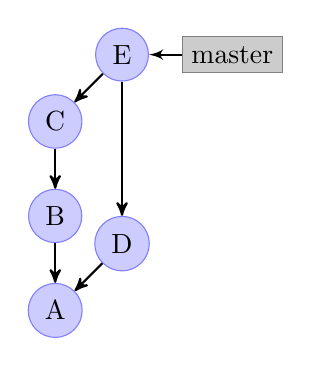
\begin{tikzpicture}[node distance=12mm]
            \node[commit] (A) {A};
            \node[commit] (B)  [above of=A] {B};
            \node[commit] (C)  [above of=B] {C};
            \path[prnt] (C) edge (B);
            \path[prnt] (B) edge (A);

            \node[commit] (D)  [above right of=A] {D};
            \path[prnt] (D) edge (A);

            \node[commit] (E)  [above right of=C] {E};
            \path[prnt] (E) edge (C);
            \path[prnt] (E) edge (D);

            \node[ref]  (m)  [right of=E,xshift=0.2cm] {master};
            \path[bptr] (m) edge (E);

        \end{tikzpicture}
        }
      \end{block}
      \column{0.60\textwidth}
      \begin{block}{Local Commit Names}
        \uncover<3->{
        \begin{itemize}
          \item E = master
          \item C = master\parent{1} = master\ancestor{1}
          \item D = master\parent{2}
          \item B = master\parent{1}\parent{1} = master\ancestor{2}
          \item A = master\ancestor{3} \quad or \quad
                A = master\parent{2}\ancestor{1}
        \end{itemize}
        }
      \end{block}
    \end{columns}
  \end{center}
  }

  \uncover<4->{
  \small
  Or, use globally unique identifiers from \cmd{git log}
  (e.g. a99816d0b6c626befb0234485b4964887faca4d5),
  their abbreviation (e.g. a99816d0b), or their \cmd{git describe}
  shorthand (e.g. 3.12.4.1-186-ga99816d0b).
  }

\end{frame}

%%%%%%%%%%%%%%%%%%%%%%%%%%%%%%%%%%%%%%%%%%%%%%%%%%%%%%%%%%%%%%%%%%%%%%%%%%
\section[Digging]{Getting information from git}
\subsection[gitk]{Viewing changes with \texttt{gitk}}
%%%%%%%%%%%%%%%%%%%%%%%%%%%%%%%%%%%%%%%%%%%%%%%%%%%%%%%%%%%%%%%%%%%%%%%%%%

\begin{frame}[fragile]
  \frametitle{Viewing Changes with \texttt{gitk}}

  \vspace*{-0.5cm}
  \begin{semiverbatim}
    \cl{gitk &}
  \end{semiverbatim}
  \vspace*{-2\baselineskip}
  \begin{center}
    %\includegraphics[height=0.62\textheight]{gitk-jgit-screenshot.png}
    \hspace*{0.1cm}
    %\includegraphics[height=0.62\textheight]{gitk-view-screenshot.png}
  \end{center}
  \vspace*{-0.3cm}
  Dialog on right from View$\rightarrow$New View (or press F4).

\end{frame}

%%%%%%%%%%%%%%%%%%%%%%%%%%%%%%%%%%%%%%%%%%%%%%%%%%%%%%%%%%%%%%%%%%%%%%%%%%
\subsection[Log]{Viewing and digging for changes with \texttt{git log}}
%%%%%%%%%%%%%%%%%%%%%%%%%%%%%%%%%%%%%%%%%%%%%%%%%%%%%%%%%%%%%%%%%%%%%%%%%%

%%%%%%%%%%%%%%%%%%%%%%%%%%%%%%%%%%%%%%%%%%%%%%%%%%%%%%%%%%%%%%%%%%%%%%%%%%

\begin{frame}[fragile]
  \frametitle{Viewing commits with \texttt{git log}}

  \only<1| handout:1>{Initial state after \cmd{git fetch}}
  \only<2| handout:2>{\cl{git log}}
  \only<3| handout:3>{\cl{git log origin/master..master}}
  \only<4| handout:4>{\cl{git log master..origin/master}}
  \only<5| handout:5>{\cl{git log origin/master...master}}
  \vspace*{-0.7cm}

  \begin{center}
    \begin{columns}[t]
      \column{0.40\textwidth}
      \begin{block}{Local clone}
        \begin{tikzpicture}[node distance=15mm]

          \only<1| handout:1>{
            \node[commit] (A) {A};
            \node[commit] (B)  [above of=A] {B};
            \node[commit] (C)  [above of=B] {C};
          }
          \only<2| handout:2>{
            \node[redCommit] (A) {A};
            \node[redCommit] (B)  [above of=A] {B};
            \node[redCommit] (C)  [above of=B] {C};
          }
          \only<3| handout:3>{
            \node[commit] (A) {A};
            \node[redCommit] (B)  [above of=A] {B};
            \node[redCommit] (C)  [above of=B] {C};
          }
          \only<4| handout:4>{
            \node[commit] (A) {A};
            \node[commit] (B)  [above of=A] {B};
            \node[commit] (C)  [above of=B] {C};
          }
          \only<5| handout:5>{
            \node[commit] (A) {A};
            \node[redCommit] (B)  [above of=A] {B};
            \node[redCommit] (C)  [above of=B] {C};
          }

          \path[prnt] (C) edge (B);
          \path[prnt] (B) edge (A);

          \node[ref]    (m)  [right of=C] {master};
          \node[ref]    (h)  [right of=m,xshift=0.8em] {HEAD};
          \path[bptr] (m) edge (C);
          \path[bptr] (h) edge (m);

          \only<1-3| handout:1-3>{
            \node[commit] (D)  [above right of=A] {D};
          }
          \only<4-5| handout:4-5>{
            \node[redCommit] (D)  [above right of=A] {D};
          }
          \node[ref]    (om) [right of=D,xshift=1.4em] {origin/master};
          \path[prnt] (D) edge (A);
          \path[bptr] (om) edge (D);

        \end{tikzpicture}
      \end{block}
      \column{0.50\textwidth}
      \only<2-| handout:2->{
        \begin{block}{log output}
          \begin{center}
            \begin{tikzpicture}[node distance=15mm]
              \only<2| handout:2>{
                \node[msg] (Am) {\texttt{commit message for A}};
                \node[msg] (Bm) [above of=Am] {\texttt{commit message for B}};
                \node[msg] (Cm) [above of=Bm] {\texttt{commit message for C}};
                \path[nextmsg] (Bm) edge (Am);
                \path[nextmsg] (Cm) edge (Bm);
              }
              \only<3| handout:3>{
                \node[msg] (Bm) {\texttt{commit message for B}};
                \node[msg] (Cm) [above of=Bm] {\texttt{commit message for C}};
                \path[nextmsg] (Cm) edge (Bm);
              }
              \only<4| handout:4>{
                \node[msg] (Dm) {\texttt{commit message for D}};
              }
              \only<5| handout:5>{
                \node[msg] (Bm) {\texttt{commit message for B}};
                \node[msg] (Dm) [above of=Bm] {\texttt{commit message for D}};
                \node[msg] (Cm) [above of=Dm] {\texttt{commit message for C}};
                \path[nextmsg] (Cm) edge (Dm);
                \path[nextmsg] (Dm) edge (Bm);
              }
            \end{tikzpicture}
          \end{center}
        \end{block}%
      }
    \end{columns}
    \only<2| handout:2>{
      \vspace*{2em}
      Shows all commits in the current branch (\textbf{master})
    }
    \only<3| handout:3>{
      \vspace*{2em}
      Shows all commits in \textbf{master} that are not
      in \textbf{origin/master}
    }
    \only<4| handout:4>{
      \vspace*{2em}
      Shows all commits in \textbf{origin/master} that are not
      in \textbf{master}
    }
    \only<5| handout:5>{
      \vspace*{2em}
      Shows all commits that are in exactly one of \textbf{origin/master}
      and \textbf{master}

      \vspace*{1em}

      log output is ordered by date, by
      default; \cmd{{-}{-}topo-order} is often helpful if you have
      lots of merges (e.g. the merges made by gerrit)

    }
  \end{center}
\end{frame}

%%%%%%%%%%%%%%%%%%%%%%%%%%%%%%%%%%%%%%%%%%%%%%%%%%%%%%%%%%%%%%%%%%%%%%%%%%

\begin{frame}[fragile]
  \frametitle{Getting more info out of \texttt{git log}}
\small

\begin{itemize}
  \item<1-> Commit Messages + Changes

    git log shows commit information only by default, but can also show the
    changes made in a commit (in diff/patch format):
    \begin{center}
      \cl{git log -p \nonliteral{$\ldots$}}
    \end{center}

  \item<2-> High level change statistics

    You can also use the same high level statistic flags as with git diff,
    instead of (or in addition to) passing the -p flag to git log:
    \cmd{{-}{-}name-only},
    \cmd{{-}{-}name-status},\,
    \cmd{{-}{-}stat},\,
    \cmd{{-}{-}dirstat}, and
    \cmd{{-}{-}shortstat}.

  \item<3-> Data Mining

    All ``View'' options from gitk (and some extras) can be accessed from
    git log; for example:
    \begin{itemize}
      \item \cmd{{-}{-}author=}\nonliteral{author regex}
      \item \cmd{{-}{-}grep=}\nonliteral{commit message regex}
      \item \cmd{{-}{-}since=}\nonliteral{date string}
      \item \cmd{{-}{-}until=}\nonliteral{date string}
      \item \cmd{-S}\nonliteral{'text to find in a file change}'
    \end{itemize}

\end{itemize}

\end{frame}

%%%%%%%%%%%%%%%%%%%%%%%%%%%%%%%%%%%%%%%%%%%%%%%%%%%%%%%%%%%%%%%%%%%%%%%%%%

\begin{frame}[fragile]
  \frametitle{Getting less info out of the log}
\small

  git log can provide a lot of information.  Sometimes, you want less ---
  just the one-line summaries, grouped by author.  In such cases, use
  shortlog.  An example:
  \begin{center}
    \cl{git shortlog 3.12.4..master}
  \end{center}

\end{frame}

%%%%%%%%%%%%%%%%%%%%%%%%%%%%%%%%%%%%%%%%%%%%%%%%%%%%%%%%%%%%%%%%%%%%%%%%%%
\subsection[Diff]{Viewing changes with \texttt{git diff}}
%%%%%%%%%%%%%%%%%%%%%%%%%%%%%%%%%%%%%%%%%%%%%%%%%%%%%%%%%%%%%%%%%%%%%%%%%%

%%%%%%%%%%%%%%%%%%%%%%%%%%%%%%%%%%%%%%%%%%%%%%%%%%%%%%%%%%%%%%%%%%%%%%%%%%

\begin{frame}[fragile]
  \frametitle{Viewing Changes with Diff (1/2) --- revisions and paths}
\small

\begin{center}
  git diff [\textsl{options}] [\textsl{FROM} [\textsl{TO}]] [{-}{-}] \textsl{PATHS}
\end{center}
\begin{itemize}
  \item \textsl{FROM} - revision specifier (or staging area if unspecified)\\
  \item \textsl{TO} - revision specifier (or working copy if unspecified)
\end{itemize}

\begin{semiverbatim}
# See the changes between HEAD and the working copy
\cl{git diff HEAD}

# See the changes between master~1 and the working copy
\cl{git diff master~1}

# See the changes between origin/master and master
\cl{git diff origin/master master}

# See the changes under framework/ since master~2
\cl{git diff master~2 {-}{-} framework}
\end{semiverbatim}

\end{frame}

%%%%%%%%%%%%%%%%%%%%%%%%%%%%%%%%%%%%%%%%%%%%%%%%%%%%%%%%%%%%%%%%%%%%%%%%%%

\begin{frame}[fragile]
  \frametitle{Viewing Changes with Diff (2/2) --- high level stats}
\small

Diff has various forms of high level statistics:
\begin{itemize}
  \item \cmd{git diff {-}{-}name-only}
        \quad\textsl{
          \# Just list the names of the changed files}
  \item \cmd{git diff {-}{-}name-status}
        \quad\textsl{
          \# Files that changed and the change type}
  \item \cmd{git diff {-}{-}stat}
        \quad\textsl{
          \# Files that changed and added/removed linecount}
  \item \cmd{git diff {-}{-}dirstat}
        \quad\textsl{
          \# List directories by percentage of line changes}
  \item \cmd{git diff {-}{-}shortstat}
        \quad\textsl{
          \# List the overall line change count}
\end{itemize}

\end{frame}

%%%%%%%%%%%%%%%%%%%%%%%%%%%%%%%%%%%%%%%%%%%%%%%%%%%%%%%%%%%%%%%%%%%%%%%%%%
\subsection[Grep]{Searching for text in files with \texttt{git grep}}
%%%%%%%%%%%%%%%%%%%%%%%%%%%%%%%%%%%%%%%%%%%%%%%%%%%%%%%%%%%%%%%%%%%%%%%%%%

%%%%%%%%%%%%%%%%%%%%%%%%%%%%%%%%%%%%%%%%%%%%%%%%%%%%%%%%%%%%%%%%%%%%%%%%%%

\begin{frame}[fragile]
  \frametitle{Searching for text in files with \texttt{git grep}}
\small

  You can look for string or regex matches in currently checked out files
  \begin{center}
    \cl{git grep \nonliteral{PATTERN}}
  \end{center}
  \uncover<2->{
  This is nicer than standard grep in that it skips executables, test
  results, and other untracked files.
  }

  \uncover<3->{
  \vspace*{\baselineskip}
  You can also search in files of a different revision
  \begin{center}
    \cl{git grep \nonliteral{PATTERN} \nonliteral{REVISION}}
  \end{center}
  }
  \uncover<4->{
  and/or search in a specific list of files and directories:
  \begin{center}
    \cl{git grep \nonliteral{PATTERN} \nonliteral{REVISION} {-}{-} \nonliteral{DIRECTORY}}
  \end{center}
  }

\end{frame}

%%%%%%%%%%%%%%%%%%%%%%%%%%%%%%%%%%%%%%%%%%%%%%%%%%%%%%%%%%%%%%%%%%%%%%%%%%
\subsection[Bisect]{Bisecting history to find a bad commit}
%%%%%%%%%%%%%%%%%%%%%%%%%%%%%%%%%%%%%%%%%%%%%%%%%%%%%%%%%%%%%%%%%%%%%%%%%%

%%%%%%%%%%%%%%%%%%%%%%%%%%%%%%%%%%%%%%%%%%%%%%%%%%%%%%%%%%%%%%%%%%%%%%%%%%
\begin{frame}[containsverbatim]
  \frametitle{Bisecting}

  Git provides a bisect command for finding the commit that introduced
  some bug through a binary search of history.

  \vspace{3mm}
  {\scriptsize{\tt
  \$ {\hilight git bisect start} {\nonliteral BAD\_REVISION GOOD\_REVISION}\\
  <Repeat until done:>\\
  ~~<Compile, link, test, see if given revision is good or bad>\\
  ~~\$ {\hilight git bisect bad}~~~~$\Leftrightarrow$~~~~\$ {\hilight git bisect good}\\
  }}
  \vspace{3mm}

  You can automate that looping step with a script that compiles,
  links, tests, and returns whether the given revision is good:

  \vspace{3mm}
  {\scriptsize{\tt
  \$ {\hilight git bisect run} {\nonliteral NAME\_OF\_SCRIPT}\\
  }}
  \vspace{3mm}

\end{frame}

%%%%%%%%%%%%%%%%%%%%%%%%%%%%%%%%%%%%%%%%%%%%%%%%%%%%%%%%%%%%%%%%%%%%%%%%%%
\subsection[Blame]{Finding where certain lines came from}
%%%%%%%%%%%%%%%%%%%%%%%%%%%%%%%%%%%%%%%%%%%%%%%%%%%%%%%%%%%%%%%%%%%%%%%%%%

%%%%%%%%%%%%%%%%%%%%%%%%%%%%%%%%%%%%%%%%%%%%%%%%%%%%%%%%%%%%%%%%%%%%%%%%%%
\begin{frame}[containsverbatim]
  \frametitle{Finding where certain lines came from}

  If you want to see which revisions introduced certain lines of
  bar.java (excluding whitespace-only changes, which is what -w is for)

  \vspace{3mm}
  {\scriptsize{\tt
  \$ {\hilight git blame -w bar.java}\\
  }}
  \vspace{3mm}

  You can do more advanced things like restrict to lines 115 through
  120, and request to also find out whether the line was introduced by
  moving or copying from some other file.

  \vspace{3mm}
  {\scriptsize{\tt
  \$ {\hilight git blame -L 115,120 -C -C -w bar.java}\\
  }}
  \vspace{3mm}

  \vspace{-2mm}
  (You can also use regexes instead of line numbers for both beginning
  and ending criteria for your range.)

  \vspace\baselineskip

  If you want to know when a certain line (or substring thereof)
  was \textit{removed}, then you need to use {\scriptsize \hilight \tt
  git log -S{\nonliteral{'SEARCH STRING'}}} (which actually checks for
  that text being added or removed).  Or you can make that search
  string a regex with {\scriptsize \hilight \tt {-}{-}pickaxe-regex}.

\end{frame}

%%%%%%%%%%%%%%%%%%%%%%%%%%%%%%%%%%%%%%%%%%%%%%%%%%%%%%%%%%%%%%%%%%%%%%%%%%
\section{Clean DAG}
\subsection[Amend]{Amending commits}
%%%%%%%%%%%%%%%%%%%%%%%%%%%%%%%%%%%%%%%%%%%%%%%%%%%%%%%%%%%%%%%%%%%%%%%%%%

%%%%%%%%%%%%%%%%%%%%%%%%%%%%%%%%%%%%%%%%%%%%%%%%%%%%%%%%%%%%%%%%%%%%%%%%%%

\begin{frame}
  \frametitle{Amending Commits}

  \only<1| handout:1>{Starting point:}
  \only<2-| handout:2>{\cl{git commit {-}{-}amend}}
  \vspace*{-0.7cm}

  \begin{center}
    \begin{columns}
      \column{0.60\textwidth}
      \begin{block}{Local repository}
        \begin{tikzpicture}[node distance=12mm]
          \only<1-| handout:1->{
            \node[commit] (A) {A};

            \node[commit] (B) [above of=A] {B};
            \path[prnt]   (B) edge (A);

            \node[ref]  (om) [right of=B,xshift=2.0em] {origin/master};
            \path[bptr] (om) edge (B);

            \node[commit] (C) [above of=B] {C};
            \path[prnt]   (C) edge (B);
          }
          \only<1| handout:1>{
            \node[commit] (D) [above of=C] {D};
            \path[prnt]   (D) edge (C);

            \node[ref]  (m) [right of=D,xshift=0.5em] {master};
            \path[bptr] (m) edge (D);

            \node[ref]  (h) [right of=m,xshift=1.3em] {HEAD};
            \path[bptr] (h) edge (m);
          }

          \only<2| handout:2>{
            \node[orphanCommit] (D) [above of=C] {D};
            \path[prnt]         (D) edge (C);

            \node[commit] (Dp) [above right of=C]{D$^*$};
            \path[prnt]   (Dp) edge (C);

            \node[ref]  (m) [right of=Dp,xshift=1.3em] {master};
            \path[bptr] (m) edge (Dp);

            \node[ref]  (h) [right of=m,xshift=1.3em] {HEAD};
            \path[bptr] (h) edge (m);
          }
        \end{tikzpicture}
      \end{block}
    \end{columns}
  \end{center}

\end{frame}

%%%%%%%%%%%%%%%%%%%%%%%%%%%%%%%%%%%%%%%%%%%%%%%%%%%%%%%%%%%%%%%%%%%%%%%%%%
\subsection{Cherry-pick}
%%%%%%%%%%%%%%%%%%%%%%%%%%%%%%%%%%%%%%%%%%%%%%%%%%%%%%%%%%%%%%%%%%%%%%%%%%

%%%%%%%%%%%%%%%%%%%%%%%%%%%%%%%%%%%%%%%%%%%%%%%%%%%%%%%%%%%%%%%%%%%%%%%%%%

\begin{frame}[fragile]
  \frametitle{Cherry-Picking Commits}

  \only<1| handout:0>{Starting point: working on topic branch ``4.0.0-pi''}
  \only<2| handout:1>{You want the changes in B (but not C) to be applied to \textbf{4.0.0-pi}}
  \only<0| handout:1>{\newline}
  \only<3-| handout:1>{\cl{git cherry-pick master$\sim$1}}

  \vspace*{-0.7cm}

  \begin{center}
    \begin{columns}[t]
      \column{0.40\textwidth}
      \begin{block}{Before cherry-pick}
        \begin{tikzpicture}[node distance=14mm]
          \node[commit] (A) {A};

          \node[commit] (D) [above right of=A] {D};
          \path[prnt]   (D) edge (A);

          \node[commit] (E) [above right of=D] {E};
          \path[prnt]   (E) edge (D);

          \only<1| handout:0>{
            \node[commit] (B) [above of=A] {B};
            \path[prnt]   (B) edge (A);

            \node[commit] (C) [above of=B] {C};
            \path[prnt]   (C) edge (B);

            \node[ref]  (c) [right of=E,xshift=0.5em] {4.0.0-pi};
            \path[bptr] (c) edge (E);

            \node[ref]  (m) [right of=C,xshift=0.5em] {master};
            \path[bptr] (m) edge (C);

            \node[ref]  (h) [below of=c] {HEAD};
            \path[bptr] (h) edge (c);
          }
          \only<2-| handout:1>{
            \node[redCommit] (B) [above of=A] {B};
            \path[prnt]   (B) edge (A);

            \node[commit] (C) [above of=B] {C};
            \path[prnt]   (C) edge (B);

            \node[ref]  (c) [right of=E,xshift=0.5em] {4.0.0-pi};
            \path[bptr] (c) edge (E);

            \node[ref]  (m) [right of=C,xshift=0.5em] {master};
            \path[bptr] (m) edge (C);

            \node[ref]  (h) [below of=c] {HEAD};
            \path[bptr] (h) edge (c);
          }
        \end{tikzpicture}
      \end{block}
      \column{0.50\textwidth}
      \only<3-| handout:1>{
        \begin{block}{After cherry-pick}
          \begin{tikzpicture}[node distance=14mm]
            \node[commit] (A) {A};

            \node[commit] (D) [above right of=A] {D};
            \path[prnt]   (D) edge (A);

            \node[commit] (E) [above right of=D] {E};
            \path[prnt]   (E) edge (D);

            \node[commit] (B) [above of=A] {B};
            \path[prnt]   (B) edge (A);

            \node[commit] (C) [above of=B] {C};
            \path[prnt]   (C) edge (B);

            \node[redCommit] (Bp) [above right of=E] {B$^*$};
            \path[prnt]   (Bp) edge (E);

            \node[ref]  (c) [right of=Bp,xshift=0.5em] {4.0.0-pi};
            \path[bptr] (c) edge (Bp);

            \node[ref]  (m) [right of=C,xshift=0.5em] {master};
            \path[bptr] (m) edge (C);

            \node[ref]  (h) [below of=c] {HEAD};
            \path[bptr] (h) edge (c);
          \end{tikzpicture}
        \end{block}
      }
    \end{columns}
    \only<3-| handout:1>{
      \vspace*{1em}
      For this usage, \cmd{git cherry-pick} will re-use the\\ commit message by default
    }
  \end{center}

\end{frame}

%%%%%%%%%%%%%%%%%%%%%%%%%%%%%%%%%%%%%%%%%%%%%%%%%%%%%%%%%%%%%%%%%%%%%%%%%%
\subsection[Revert]{Make a new change that undoes a former one}
%%%%%%%%%%%%%%%%%%%%%%%%%%%%%%%%%%%%%%%%%%%%%%%%%%%%%%%%%%%%%%%%%%%%%%%%%%

%%%%%%%%%%%%%%%%%%%%%%%%%%%%%%%%%%%%%%%%%%%%%%%%%%%%%%%%%%%%%%%%%%%%%%%%%%

\begin{frame}[fragile]
  \frametitle{Reverting Commits}

  \only<1| handout:0>{Starting point: working on topic branch ``4.0.0-pi''}
  \only<2| handout:1>{You want to reverse apply the changes in B (but not C)}
  \only<0| handout:1>{\newline}
  \only<3-| handout:1>{\cl{git revert 4.0.0-pi$\sim$1}}

  \vspace*{-0.7cm}

  \begin{center}
    \begin{columns}[t]
      \column{0.40\textwidth}
      \begin{block}{Before revert}
        \begin{tikzpicture}[node distance=12mm]
          \node[commit] (A) {A};

          \only<1| handout:0>{
            \node[commit] (B) [above of=A] {B};
            \path[prnt]   (B) edge (A);

            \node[commit] (C) [above of=B] {C};
            \path[prnt]   (C) edge (B);

            \node[ref]  (c) [right of=C,xshift=1em] {4.0.0-pi};
            \path[bptr] (c) edge (C);

            \node[ref]  (h) [right of=c,xshift=1em] {HEAD};
            \path[bptr] (h) edge (c);
          }
          \only<2-| handout:1>{
            \node[redCommit] (B) [above of=A] {B};
            \path[prnt]   (B) edge (A);

            \node[commit] (C) [above of=B] {C};
            \path[prnt]   (C) edge (B);

            \node[ref]  (c) [right of=C,xshift=1em] {4.0.0-pi};
            \path[bptr] (c) edge (C);

            \node[ref]  (h) [right of=c,xshift=1em] {HEAD};
            \path[bptr] (h) edge (c);
          }
        \end{tikzpicture}
      \end{block}
      \column{0.50\textwidth}
      \only<3-| handout:1>{
        \begin{block}{After revert}
          \begin{tikzpicture}[node distance=12mm]
            \node[commit] (A) {A};
            \node[commit] (B) [above of=A] {B};
            \path[prnt]   (B) edge (A);

            \node[commit] (C) [above of=B] {C};
            \path[prnt]   (C) edge (B);

            \node[redCommit] (Bi) [above of=C] {B$^{-1}$};
            \path[prnt]   (Bi) edge (C);

            \node[ref]  (c) [right of=Bi,xshift=1em] {4.0.0-pi};
            \path[bptr] (c) edge (Bi);

            \node[ref]  (h) [right of=c,xshift=1em] {HEAD};
            \path[bptr] (h) edge (c);
          \end{tikzpicture}
        \end{block}
      }
    \end{columns}
    \only<3-| handout:1>{
      \vspace*{1em}
      \cmd{git revert} will prompt for a new commit message
    }
  \end{center}

\end{frame}

%%%%%%%%%%%%%%%%%%%%%%%%%%%%%%%%%%%%%%%%%%%%%%%%%%%%%%%%%%%%%%%%%%%%%%%%%%
\subsection[Reset]{Undoing and redoing commits}
%%%%%%%%%%%%%%%%%%%%%%%%%%%%%%%%%%%%%%%%%%%%%%%%%%%%%%%%%%%%%%%%%%%%%%%%%%

%%%%%%%%%%%%%%%%%%%%%%%%%%%%%%%%%%%%%%%%%%%%%%%%%%%%%%%%%%%%%%%%%%%%%%%%%%

\begin{frame}
  \frametitle{Undoing/Redoing Commits}

  \only<1| handout:1>{Starting point:}
  \only<2| handout:2>{\cl{git reset {-}{-}hard origin/master}}
  \only<3| handout:3>{\cl{git reset {-}{-}hard ORIG\_HEAD}}
  \only<4| handout:4>{\cl{git pull}}
  \only<5| handout:5>{\cl{git reset {-}{-}hard ORIG\_HEAD}}
  \only<6| handout:6>{\cl{git reset {-}{-}hard master\ancestor{1}}}
  \only<7| handout:0>{\cl{git reset {-}{-}hard master@\{4\}}}
  \only<8| handout:0>{\cl{git reset {-}{-}hard master@\{``30 seconds ago''\}}}
  \vspace*{-0.7cm}

  \begin{center}
    \begin{columns}
      \column{0.65\textwidth}
      \begin{block}{Local repository}
        \begin{tikzpicture}[node distance=12mm]
          \only<1-| handout:1->{
            \node[commit] (A) {A};

            \node[commit] (B) [above of=A] {B};
            \path[prnt]   (B) edge (A);

            \node[ref]  (om) [right of=B,xshift=2.0em] {origin/master};
            \path[bptr] (om) edge (B);
          }

          \only<1,3-6,8| handout:1,3-6>{
            \node[commit] (C) [above of=B] {C};
            \path[prnt]   (C) edge (B);
          }
          \only<2,7| handout:2>{
            \node[orphanCommit] (C) [above of=B] {C};
            \path[prnt]   (C) edge (B);
          }

          \only<1,3-5,8| handout:1,3-5>{
            \node[commit] (E) [above of=C] {E};
            \path[prnt]   (E) edge (C);
          }
          \only<2,6-7| handout:2,6>{
            \node[orphanCommit] (E) [above of=C] {E};
            \path[prnt]   (E) edge (C);
          }

          \only<1,3| handout:1,3>{
            \node[ref]  (m) [right of=E,xshift=0.5em] {master};
            \path[bptr] (m) edge (E);

            \node[ref]  (h) [right of=m,xshift=1.3em] {HEAD};
            \path[bptr] (h) edge (m);
          }
          \only<2,7| handout:2>{
            \node[ref]  (m) [right of=om,xshift=2.5em] {master};
            \path[bptr] (m) edge[bend left] (B);

            \node[ref]  (h) [right of=m,xshift=1.3em] {HEAD};
            \path[bptr] (h) edge (m);
          }
          \only<4,8| handout:4>{
            \node[commit] (D) [above right of=B] {D};
            \path[prnt]   (D) edge (B);

            \node[commit] (F) [above right of=D] {F};
            \path[prnt]   (F) edge (D);

            \node[commit] (G) [above left of=F,xshift=0.5em] {G};
            \path[prnt]   (G) edge (E);
            \path[prnt]   (G) edge (F);
          }
          \only<5-7| handout:5-6>{
            \node[orphanCommit] (D) [above right of=B] {D};
            \path[prnt]   (D) edge (B);

            \node[orphanCommit] (F) [above right of=D] {F};
            \path[prnt]   (F) edge (D);

            \node[orphanCommit] (G) [above left of=F,xshift=0.5em] {G};
            \path[prnt]   (G) edge (E);
            \path[prnt]   (G) edge (F);
          }
          \only<4-6,8| handout:4-6>{
            \node[ref]  (m) [right of=G,xshift=0.5em,yshift=1.1em] {master};
            \node[ref]  (h) [right of=m,xshift=1.3em] {HEAD};
            \path[bptr] (h) edge (m);
          }
          \only<4,8| handout:4>{
            \path[bptr] (m) edge (G);
          }
          \only<5| handout:5>{
            \path[bptr] (m) edge[bend right] (E);
          }
          \only<6| handout:6>{
            \path[bptr] (m) edge (C);
          }
          \only<7| handout:0>{
            \path[bptr] (m) edge[bend left] (B);
          }

          \only<1-| handout:1->{
            \node[specialRef] (oh) [above right of=E,xshift=14.0em]{ORIG\_HEAD};
          }
          \only<2| handout:2>{
            \path[bptr]       (oh) edge (E);
          }
          \only<3,8| handout:3>{
            \path[bptr]       (oh) edge (B);
          }
          \only<4,6| handout:4,6>{
            \path[bptr]       (oh) edge[bend right] (E);
          }
          \only<5| handout:5>{
            \path[bptr]       (oh) edge[bend left] (G);
          }
          \only<7| handout:0>{
            \path[bptr]       (oh) edge[bend left] (C);
          }
        \end{tikzpicture}
      \end{block}
    \end{columns}
  \end{center}

  \begin{center}
    \only<2| handout:2>{
      \texttt{{-}{-}hard}: Make sure the working copy exactly
      matches the specified commit.
    }
    \only<3-5| handout:3-5>{
      \vspace*{-0.5em}
      \texttt{ORIG\_HEAD}: set by merge, rebase, and reset.
    }
    \only<7-8| handout:0>{
      To see where master previously pointed, run\\\cmd{git reflog show [{-}{-}date=local] master}
    }
  \end{center}

\end{frame}

%%%%%%%%%%%%%%%%%%%%%%%%%%%%%%%%%%%%%%%%%%%%%%%%%%%%%%%%%%%%%%%%%%%%%%%%%%
\subsection[Squashing]{Squashing commits together}
%%%%%%%%%%%%%%%%%%%%%%%%%%%%%%%%%%%%%%%%%%%%%%%%%%%%%%%%%%%%%%%%%%%%%%%%%%

%%%%%%%%%%%%%%%%%%%%%%%%%%%%%%%%%%%%%%%%%%%%%%%%%%%%%%%%%%%%%%%%%%%%%%%%%%

\begin{frame}
  \frametitle{Squashing}

  \only<1| handout:1>{Starting point:}
  \only<2-| handout:2>{\cl{git reset {-}{-}soft origin/master \&\& git commit}}
  \vspace*{-0.7cm}

  \begin{center}
    \begin{columns}
      \column{0.60\textwidth}
      \begin{block}{Local repository}
        \begin{tikzpicture}[node distance=12mm]
          \only<1-| handout:1->{
            \node[commit] (A) {A};

            \node[commit] (B) [above of=A] {B};
            \path[prnt]   (B) edge (A);

            \node[commit] (C) [above of=B] {C};
            \path[prnt]   (C) edge (B);

            \node[commit] (D) [above right of=A] {D};
            \path[prnt]   (D) edge (A);

            \node[commit] (E) [above right of=C] {E};
            \path[prnt]   (E) edge (C);
            \path[prnt]   (E) edge (D);

            \node[ref]  (om) [right of=D,xshift=2.0em] {origin/master};
            \path[bptr] (om) edge (D);
          }
          \only<1-2| handout:1>{
            \node[ref]  (m) [right of=E,xshift=0.5em] {master};
            \path[bptr] (m) edge (E);

            \node[ref]  (h) [right of=m,xshift=1.3em] {HEAD};
            \path[bptr] (h) edge (m);
          }
          \only<2-| handout:2>{
                                         % shift={(angle-rotation:length)}
            \draw[rotate=70] (node cs:name=C) +(275:0.8em)
                  [opacity=0.7,draw=green!80,fill=green!20]
                  ellipse (4.5em and 2em);
          }

          \only<3| handout:2>{
            \node[commit] (BCEp) [above right of=D,shift={(45:0.8em)}]{BCE$^*$};
            \path[prnt]   (BCEp) edge (D);

            \node[ref]  (m) [right of=BCEp,xshift=1.3em] {master};
            \path[bptr] (m) edge (BCEp);

            \node[ref]  (h) [right of=m,xshift=1.3em] {HEAD};
            \path[bptr] (h) edge (m);
          }
        \end{tikzpicture}
      \end{block}
    \end{columns}
  \end{center}

\end{frame}

%%%%%%%%%%%%%%%%%%%%%%%%%%%%%%%%%%%%%%%%%%%%%%%%%%%%%%%%%%%%%%%%%%%%%%%%%%
\subsection[Rebase]{Rebasing (replaying) sequences of commits}
%%%%%%%%%%%%%%%%%%%%%%%%%%%%%%%%%%%%%%%%%%%%%%%%%%%%%%%%%%%%%%%%%%%%%%%%%%

%%%%%%%%%%%%%%%%%%%%%%%%%%%%%%%%%%%%%%%%%%%%%%%%%%%%%%%%%%%%%%%%%%%%%%%%%%

\begin{frame}
  \frametitle{Rebasing}

  \only<1| handout:1>{Starting point:}
  \only<2-| handout:2>{\cl{git rebase origin/master}}
  \vspace*{-0.7cm}

  \begin{center}
    \begin{columns}
      \column{0.6\textwidth}
      \begin{block}{Local repository}
        \begin{tikzpicture}[node distance=12mm]
          \only<1-| handout:1->{
            \node[commit] (A) {A};

            \node[commit] (B) [above of=A] {B};
            \path[prnt]   (B) edge (A);

            \node[commit] (C) [above of=B] {C};
            \path[prnt]   (C) edge (B);

            \node[commit] (D) [above right of=A] {D};
            \path[prnt]   (D) edge (A);

            \node[commit] (E) [above right of=C] {E};
            \path[prnt]   (E) edge (C);
            \path[prnt]   (E) edge (D);

            \node[ref]  (om) [right of=D,xshift=2.0em] {origin/master};
            \path[bptr] (om) edge (D);
          }
          \only<1-5| handout:1>{
            \node[ref]  (m) [right of=E,xshift=0.5em] {master};
            \path[bptr] (m) edge (E);
          }
          \only<1-2| handout:1>{
            \node[ref]  (h) [right of=m,xshift=1.3em] {HEAD};
            \path[bptr] (h) edge (m);
          }
          \only<2-| handout:2>{
                                         % shift={(angle-rotation:length)}
            \draw[rotate=70] (node cs:name=C) +(275:0.8em)
                  [opacity=0.7,draw=green!80,fill=green!20]
                  ellipse (4.5em and 2em);
          }

          \only<3| handout:0>{
            \node[ref]  (h) [above right of=D,xshift=1.1em] {HEAD};
            \path[bptr] (h) edge (D);
          }

          \only<4-| handout:2>{
            \node[commit] (Bp) [above right of=D] {B$^*$};
            \path[prnt]   (Bp) edge (D);
          }
          \only<4| handout:0>{
            \node[ref]  (h) [right of=Bp,xshift=0.5em] {HEAD};
            \path[bptr] (h) edge (Bp);
          }

          \only<5-| handout:2>{
            \node[commit] (Cp) [above right of=Bp] {C$^*$};
            \path[prnt]   (Cp) edge (Bp);
          }
          \only<5| handout:0>{
            \node[ref]  (h) [right of=Cp,xshift=0.5em] {HEAD};
            \path[bptr] (h) edge (Cp);
          }

          \only<6-| handout:2>{
            \node[ref]  (m) [right of=Cp,xshift=0.8em] {master};
            \path[bptr] (m) edge (Cp);

            \node[ref]  (h) [right of=m,xshift=1.2em] {HEAD};
            \path[bptr] (h) edge (m);
          }
        \end{tikzpicture}
      \end{block}
    \end{columns}
  \end{center}

  \only<6-7| handout:2>{
  \uncover<7| handout:2>{
    \begin{center}
      Merge commits are dropped during rebases, so E is not applied.
    \end{center}
  }}

\end{frame}

%%%%%%%%%%%%%%%%%%%%%%%%%%%%%%%%%%%%%%%%%%%%%%%%%%%%%%%%%%%%%%%%%%%%%%%%%%

\begin{frame}[fragile]
  \frametitle{Interactive Rebasing}

  \only<1| handout:0>{Starting point:}
  \only<2-| handout:1>{\cl{git rebase {-}{-}interactive origin/master}}
  \vspace*{-0.7cm}

  \begin{center}
    \begin{columns}[t]
      \column{0.30\textwidth}
      \begin{block}{Local repository}
        \begin{tikzpicture}[node distance=10mm]
          \only<1-2| handout:0>{
            \node[commit] (A) {\tiny A};

            \node[commit] (B) [above of=A] {\tiny B};
            \path[prnt]   (B) edge (A);

            \node[commit] (C) [above of=B] {\tiny C};
            \path[prnt]   (C) edge (B);

            \node[commit] (D) [above of=C] {\tiny D};
            \path[prnt]   (D) edge (C);

            \node[commit] (E) [above right of=A] {\tiny E};
            \path[prnt]   (E) edge (A);

            \node[commit] (F) [above right of=D] {\tiny F};
            \path[prnt]   (F) edge (D);
            \path[prnt]   (F) edge (E);

            \node[ref]  (om) [right of=E,xshift=1em] {\tiny origin/master};
            \path[bptr] (om) edge (E);

            \node[ref]  (m) [right of=F,xshift=0.5em] {\tiny master};
            \path[bptr] (m) edge (F);

            \node[ref]  (h) [above of=m] {\tiny HEAD};
            \path[bptr] (h) edge (m);
          }
          \only<3-4| handout:1>{
            \node[commit] (A) {\tiny A};

            \node[redCommit] (B) [above of=A] {\tiny B};
            \path[prnt]   (B) edge (A);

            \node[redCommit] (C) [above of=B] {\tiny C};
            \path[prnt]   (C) edge (B);

            \node[redCommit] (D) [above of=C] {\tiny D};
            \path[prnt]   (D) edge (C);

            \node[commit] (E) [above right of=A] {\tiny E};
            \path[prnt]   (E) edge (A);

            \node[droppedCommit] (F) [above right of=D] {\tiny F};
            \path[prnt]   (F) edge (D);
            \path[prnt]   (F) edge (E);

            \node[ref]  (om) [right of=E,xshift=1em] {\tiny origin/master};
            \path[bptr] (om) edge (E);

            \node[ref]  (m) [right of=F,xshift=0.5em] {\tiny master};
            \path[bptr] (m) edge (F);

            \node[ref]  (h) [above of=m] {\tiny HEAD};
            \path[bptr] (h) edge (m);
          }
          \only<5-| handout:2>{
            \node[commit] (A) {\tiny A};

            \node[orphanCommit] (B) [above of=A] {\tiny B};
            \path[oprnt]   (B) edge (A);

            \node[orphanCommit] (C) [above of=B] {\tiny C};
            \path[oprnt]   (C) edge (B);

            \node[orphanCommit] (D) [above of=C] {\tiny D};
            \path[oprnt]   (D) edge (B);

            \node[commit] (E) [above right of=A] {\tiny E};
            \path[prnt]   (E) edge (A);

            \node[orphanCommit] (F) [above right of=D] {\tiny F};
            \path[oprnt]   (F) edge (D);
            \path[oprnt]   (F) edge (E);

            \node[commit] (Dp) [above right of=E] {\tiny D$^*$};
            \path[prnt]   (Dp) edge (E);

            \node[commit] (BCp) [above of=Dp] {\tiny BC$^*$};
            \path[prnt]   (BCp) edge (Dp);

            \node[ref]  (om) [right of=E,xshift=1em] {\tiny origin/master};
            \path[bptr] (om) edge (E);

            \node[ref]  (m) [right of=BCp,xshift=0.5em] {\tiny master};
            \path[bptr] (m) edge (BCp);

            \node[ref]  (h) [above of=m] {\tiny HEAD};
            \path[bptr] (h) edge (m);
          }
        \end{tikzpicture}
      \end{block}
      \column{0.65\textwidth}
      \only<1| handout:0>{
        \begin{block}{Terminal}
          \begin{semiverbatim}\scriptsize
            \cl{ }
          \end{semiverbatim}
        \end{block}
      }
      \only<2| handout:0>{
        \begin{block}{Terminal}
          \begin{semiverbatim}\scriptsize
            \cl{git rebase -i origin/master}
          \end{semiverbatim}
        \end{block}
      }
      \only<3| handout:0>{
        \begin{block}{Editor}
          \begin{semiverbatim}\tiny
            \Red{pick b6bafc0 Commit message B}\newline
            \Red{pick 44a6ae8 Commit message C}\newline
            \Red{pick 238ea47 Commit message D}\newline

            \# Rebase e67fc45..fc16033 onto e67fc45\newline
            \#\newline
            \# Commands:\newline
            \#  p, pick = use commit\newline
            \#  e, edit = use commit, but stop for amending\newline
            \#  s, squash = use commit, but meld into previous commit\newline
            \#\newline
            \# If you remove a line here THAT COMMIT WILL BE LOST.\newline
            \# However, if you remove everything, the rebase will be aborted.\newline
            \#
          \end{semiverbatim}
        \end{block}
      }
      \only<4| handout:1>{
        \begin{block}{Editor}
          \begin{semiverbatim}\tiny
            \Red{pick 238ea47 Commit message D}\newline
            \Red{pick b6bafc0 Commit message B}\newline
            \Red{squash 44a6ae8 Commit message C}\newline

            \# Rebase e67fc45..fc16033 onto e67fc45\newline
            \#\newline
            \# Commands:\newline
            \#  p, pick = use commit\newline
            \#  e, edit = use commit, but stop for amending\newline
            \#  s, squash = use commit, but meld into previous commit\newline
            \#\newline
            \# If you remove a line here THAT COMMIT WILL BE LOST.\newline
            \# However, if you remove everything, the rebase will be aborted.\newline
            \#
          \end{semiverbatim}
        \end{block}
      }
      \only<4| handout:1>{
        \vspace*{-1em}
        \small
        \begin{enumerate}
        \item Move commit D to the top
        \item Change commit C from \textbf{pick} to \textbf{squash}
        \item Save and exit editor
        \end{enumerate}
      }
      \only<5| handout:2>{
        \begin{block}{Editor}
          \begin{semiverbatim}\tiny
            \# This is a combination of two commits.\newline
            \# The first commit's message is:\newline

            \Red{Commit message B}\newline

            \# This is the 2nd commit message:\newline

            \Red{Commit message C}\newline

            \# Please enter the commit message for your changes. Lines starting\newline
            \# with '\#' will be ignored, and an empty message aborts the commit.\newline
            \# Not currently on any branch.\newline
            \# Changes to be committed:\newline
            \#   (use "git reset HEAD <file>..." to unstage)\newline
            \#\newline
            \#       modified:   A\newline
            \#\newline
          \end{semiverbatim}
        \end{block}
        \vspace*{-1em}
        {\small
          \begin{enumerate}
          \item Edit commit message for the combined commit
          \item Save and exit editor
          \end{enumerate}
        }
      }
    \end{columns}
  \end{center}

\end{frame}

%%%%%%%%%%%%%%%%%%%%%%%%%%%%%%%%%%%%%%%%%%%%%%%%%%%%%%%%%%%%%%%%%%%%%%%%%%
\section[Tools]{Tools and miscellaneous tips}
%%%%%%%%%%%%%%%%%%%%%%%%%%%%%%%%%%%%%%%%%%%%%%%%%%%%%%%%%%%%%%%%%%%%%%%%%%

%%%%%%%%%%%%%%%%%%%%%%%%%%%%%%%%%%%%%%%%%%%%%%%%%%%%%%%%%%%%%%%%%%%%%%%%%%
\subsection{Stash}
\begin{frame}[fragile]
  \frametitle{The Git Stash}

  \begin{block}{Motivation}
    You want save off your uncommitted changes to clear out your
    working copy but you're not ready to do a commit.
  \end{block}

  \pause
  \vspace*{1em}

  \textbf{Sometimes you want to}
  \begin{itemize}[<+->]
  \item safely do a pull\ldots
  \item switch to another branch to work on something else\ldots
  \item experiment with different changes\ldots
  \end{itemize}
  \uncover<+->{
    \ldots without making a commit.
  }

  \pause

  \vspace*{1em}
  \uncover<+->{
    \begin{center}
      You're looking for \cmd{git stash}
    \end{center}
  }

\end{frame}

%%%%%%%%%%%%%%%%%%%%%%%%%%%%%%%%%%%%%%%%%%%%%%%%%%%%%%%%%%%%%%%%%%%%%%%%%%

\begin{frame}[fragile]
  \frametitle{Using the Stash (1/2)}

\begin{uncoverenv}<+->
\begin{semiverbatim}\scriptsize
\cl{git status}
On branch master
Changes to be committed:
  (use "git reset HEAD <file>..." to unstage)

        modified:   launch-codes.C

Changes not staged for commit:
  (use "git add <file>..." to update what will be committed)
  (use "git checkout -- <file>..." to discard changes in working directory)

        modified:   mrs-fields-cookie-recipe.C
\end{semiverbatim}
\end{uncoverenv}

\begin{uncoverenv}<+->
\begin{semiverbatim}\scriptsize
\cl{git stash}
Saved working directory and index state "WIP on master: 51cc474 Initial import"
HEAD is now at 51cc474 Initial import
(To restore them type "git stash apply")
\end{semiverbatim}
\end{uncoverenv}

\begin{uncoverenv}<+->
\begin{semiverbatim}\scriptsize
\cl{git stash list}
stash@\{0\}: WIP on master: 51cc474 Initial import
\end{semiverbatim}
\end{uncoverenv}

\end{frame}

%%%%%%%%%%%%%%%%%%%%%%%%%%%%%%%%%%%%%%%%%%%%%%%%%%%%%%%%%%%%%%%%%%%%%%%%%%

\begin{frame}[fragile]
  \frametitle{Using the Stash (2/2)}

\begin{semiverbatim}\scriptsize
\cl{git stash pop}
On branch master
Changes to be committed:
        modified:   launch-codes.C
Changes not staged for commit:
        modified:   mrs-fields-cookie-recipe.C

Dropped refs/stash@\{0\} (67abba2a0c6a8de8f0416e6757bdc73e86c15dd1)
\end{semiverbatim}

\end{frame}

%%%%%%%%%%%%%%%%%%%%%%%%%%%%%%%%%%%%%%%%%%%%%%%%%%%%%%%%%%%%%%%%%%%%%%%%%%

\begin{frame}[fragile]
  \frametitle{Multiple Stashes (1/2)}

You can have multiple stashes:\pause
\begin{uncoverenv}<+->
\begin{semiverbatim}\scriptsize
# edit some files...
\cl{git status}
On branch master
Changes not staged for commit:
    modified:  launch-codes.C
\cl{git stash save Working on ROT13 encryption}\ \  \textsl{\textbf{\usebeamercolor[fg]{item}\# some meaningful message}}
Saved working directory and index state "On master: Working on ROT13 ecryption"
HEAD is now at 51cc474 Initial import
\cl{git status}
(On branch master)
\end{semiverbatim}
\end{uncoverenv}

\begin{uncoverenv}<+->
\begin{semiverbatim}\scriptsize
# edit some files...
\cl{git status}
On branch master
Changes not staged for commit:
    modified:  mrs-fields-cookie-recipe.C
\cl{git stash save Adding more chocolate chips}
Saved working directory and index state "On master: Adding more chocolate chips"
HEAD is now at 51cc474 Initial import
\cl{git status}
(On branch master)
\end{semiverbatim}
\end{uncoverenv}

\end{frame}

%%%%%%%%%%%%%%%%%%%%%%%%%%%%%%%%%%%%%%%%%%%%%%%%%%%%%%%%%%%%%%%%%%%%%%%%%%

\begin{frame}[fragile]
  \frametitle{Multiple Stashes (2/2)}

\begin{uncoverenv}<+->
\begin{semiverbatim}\scriptsize
\cl{git stash list}
stash@\{1\}: Adding more chocolate chips: 51cc474 Initial import
stash@\{0\}: Working on ROT13 encryption on master: 51cc474 Initial import
\end{semiverbatim}
\end{uncoverenv}

\begin{uncoverenv}<+->
\begin{semiverbatim}\scriptsize
\cl{git stash apply stash@\{0\}}
On branch master
Changes not staged for commit:

        modified:   launch-codes.C
\end{semiverbatim}
\end{uncoverenv}

\begin{uncoverenv}<+->
\begin{semiverbatim}\scriptsize
\cl{git stash list}
stash@\{1\}: Adding more chocolate chips: 51cc474 Initial import
stash@\{0\}: Working on ROT13 encryption on master: 51cc474 Initial import
\end{semiverbatim}
\end{uncoverenv}

\begin{uncoverenv}<+->
\begin{semiverbatim}\scriptsize
# Find more examples and options
\cl{git help stash}
...
\end{semiverbatim}
\end{uncoverenv}
\end{frame}

%%%%%%%%%%%%%%%%%%%%%%%%%%%%%%%%%%%%%%%%%%%%%%%%%%%%%%%%%%%%%%%%%%%%%%%%%%
\subsection{Ignoring files}
%%%%%%%%%%%%%%%%%%%%%%%%%%%%%%%%%%%%%%%%%%%%%%%%%%%%%%%%%%%%%%%%%%%%%%%%%%

\begin{frame}[fragile]
  \frametitle{Ignoring Files}
\small

Git provides three mechanisms for ignoring files
\begin{itemize}
  \item \texttt{.gitignore} files -- can be checked-in and shared via repository
  \item \texttt{\$GIT\_DIR/info/excludes} file -- local to a
    project/clone (personal)
  \item \texttt{core.excludesfile} configuration paramter -- can be
    per-project or global (personal)
\end{itemize}

\uncover<2->{
  \begin{block}{Common usage}
    Setup a \texttt{$\sim$/.gitignore} file for all your Git projects
    \uncover<3->{
      \begin{semiverbatim}
      \cl{echo checkin-comments.txt > $\sim$/.gitignore}

      \cl{echo /tests/ {>}{>} $\sim$/.gitignore}

      \cl{echo \\*.bak {>}{>} $\sim$/.gitignore}

      \cl{git config {-}{-}global core.excludesfile $\sim$/.gitignore}
      \end{semiverbatim}
    }
  \end{block}
}

\end{frame}

%%%%%%%%%%%%%%%%%%%%%%%%%%%%%%%%%%%%%%%%%%%%%%%%%%%%%%%%%%%%%%%%%%%%%%%%%%
\subsection[Remotes]{Direct collaboration}
%%%%%%%%%%%%%%%%%%%%%%%%%%%%%%%%%%%%%%%%%%%%%%%%%%%%%%%%%%%%%%%%%%%%%%%%%%

%%%%%%%%%%%%%%%%%%%%%%%%%%%%%%%%%%%%%%%%%%%%%%%%%%%%%%%%%%%%%%%%%%%%%%%%%%

\begin{frame}
  \frametitle{Direct Collaboration (Remotes)}

  \only<1-2| handout:1>{Initial State:}
  \only<3| handout:0>{\cl{git remote add jim \nonliteral{machine:/PATH...}}}
  \only<4| handout:0>{\cl{git fetch jim}}
  \only<0| handout:2>{\cl{git remote add jim \nonliteral{machine:/PATH} \&\& git fetch jim}}
  \only<5| handout:0>{\cl{git remote rm origin}}
  \only<6| handout:0>{\cl{git remote rename jim origin}}
  \only<0| handout:3>{\cl{git remote rm origin \&\& git remote rename jim origin}}
  \only<7| handout:4>{Use \cmd{git remote -v} to see remotes.}
  \vspace*{-0.7cm}

  \begin{center}
    \begin{columns}[t]
      \column{0.30\textwidth}
      \begin{block}{gerrit}
        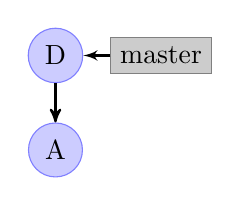
\begin{tikzpicture}[node distance=12mm]
          \node[commit] (A) {A};

          \node[commit] (D) [above of=A] {D};
          \path[prnt]   (D) edge (A);

          \node[ref]    (m) [right of=D,xshift=0.4em] {master};
          \path[bptr]   (m) edge (D);
        \end{tikzpicture}
      \end{block}%
      \uncover<2-| handout:2->{
      \begin{block}{Jim's clone}
        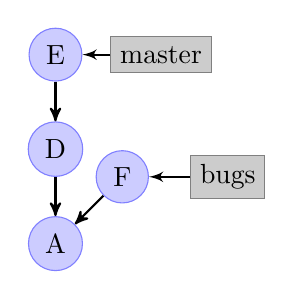
\begin{tikzpicture}[node distance=12mm]
          \node[commit] (A) {A};

          \node[commit] (D) [above of=A] {D};
          \path[prnt]   (D) edge (A);

          \node[commit] (E) [above of=D] {E};
          \path[prnt]   (E) edge (D);

          \node[ref]    (m) [right of=E,xshift=0.4em] {master};
          \path[bptr]   (m) edge (E);

          \node[commit] (F) [above right of=A] {F};
          \path[prnt]   (F) edge (A);

          \node[ref]    (b) [right of=F,xshift=0.4em] {bugs};
          \path[bptr]   (b) edge (F);
        \end{tikzpicture}
      \end{block}%
      }
      \column{0.60\textwidth}
      \begin{block}{Local clone}
        \begin{tikzpicture}[node distance=15mm]

          \node[commit] (A) {A};

          \node[commit] (B) [above of=A] {B};
          \path[prnt]   (B) edge (A);

          \node[commit] (C) [above of=B] {C};
          \path[prnt]   (C) edge (B);

          \node[ref]  (m) [above right of=C,xshift=0.4em] {master};
          \path[bptr] (m) edge (C);

          \node[ref]  (h) [right of=m,xshift=1.1em] {HEAD};
          \path[bptr] (h) edge (m);

          \only<1-4| handout:1-2>{
            \node[ref]  (om) [right of=A,xshift=1.8em] {origin/master};
            \path[bptr] (om) edge (A);
          }
          \only<4-| handout:2->{
            \node[commit] (D) [above right of=A] {D};
            \path[prnt]   (D) edge (A);

            \node[commit] (E) [above of=D] {E};
            \path[prnt]   (E) edge (D);

            \node[commit] (F) [right of=D] {F};
            \path[prnt]   (F) edge (A);
          }
          \only<4-5| handout:2>{
            \node[ref]    (jm) [right of=E,xshift=0.4em] {jim/master};
            \path[bptr]   (jm) edge (E);

            \node[ref]    (jb) [right of=F,xshift=0.4em] {jim/bugs};
            \path[bptr]   (jb) edge (F);
          }
          \only<6-7| handout:3-4>{
            \node[ref]    (jm) [right of=E,xshift=1.2em] {origin/master};
            \path[bptr]   (jm) edge (E);

            \node[ref]    (jb) [right of=F,xshift=0.7em] {origin/bugs};
            \path[bptr]   (jb) edge (F);
          }
        \end{tikzpicture}
      \end{block}
    \end{columns}
  \end{center}

\end{frame}

%%%%%%%%%%%%%%%%%%%%%%%%%%%%%%%%%%%%%%%%%%%%%%%%%%%%%%%%%%%%%%%%%%%%%%%%%%

\mode<beamer>{
  \begin{frame}
    \frametitle{}
    \vfill
    \begin{center}
      {\Large\textbf{Questions?}}
    \end{center}
    %\vfill
    %{\tiny\Hidden{\input{VERSION-FILE}}}
  \end{frame}
}
\end{comment}

%%%%%%%%%%%%%%%%%%%%%%%%%%%%%%%%%%%%%%%%%%%%%%%%%%%%%%%%%%%%%%%%%%%%%%%%%%

\end{document}
